
\documentclass[a4paper,12pt]{article}

% ============================================================
% 1. PACKAGES
% ============================================================

% Vietnamese support
\usepackage{vntex}

% Page layout
\usepackage[
    a4paper,
    left=3cm,
    right=2.5cm,
    top=2.5cm,
    bottom=2.5cm,
    headheight=38pt,
    headsep=12pt,
    footskip=18pt
]{geometry}

% Mathematics
\usepackage{amsmath,amssymb,latexsym}

% Figures and tables
\usepackage{graphicx}
\usepackage{epsfig}
\usepackage{booktabs}
\usepackage{tabularx}
\usepackage{array}
\usepackage{multirow}
\usepackage{hhline}
\usepackage{float}
\usepackage{caption}
\usepackage{rotating}

% Typography and spacing
\usepackage{indentfirst}
\usepackage{setspace}
\usepackage[shortlabels]{enumitem}
\usepackage{titlesec}
\usepackage{multicol}

% Headers and footers
\usepackage{fancyhdr}
\usepackage{lastpage}

% Algorithms and source code
\usepackage[lined,boxed,commentsnumbered]{algorithm2e}
\usepackage{xcolor}
\usepackage{listings}
\usepackage{tikz}
\usepackage[framemethod=tikz]{mdframed}

% Dates and hyperlinks
\usepackage{datetime2}
\usepackage{hyperref}

\usetikzlibrary{arrows,snakes,backgrounds}

\hypersetup{
    colorlinks=true,
    linkcolor=black,
    citecolor=black,
    urlcolor=blue
}

% ============================================================
% 2. DOCUMENT TYPOGRAPHY
% ============================================================

% Line spacing
\setstretch{1.2}

% Paragraph indentation
\setlength{\parindent}{1.25cm}

% Space between paragraphs
\setlength{\parskip}{0.2em}

% Avoid widows and orphans
\widowpenalty=10000
\clubpenalty=10000

% ============================================================
% 3. SECTION AND SUBSECTION FORMATTING
% ============================================================

% Section formatting
\titleformat{\section}
    {\normalfont\Large\bfseries}
    {\thesection}
    {0.8em}
    {}

% Subsection formatting
\titleformat{\subsection}
    {\normalfont\large\bfseries}
    {\thesubsection}
    {0.8em}
    {}

% Subsubsection formatting
\titleformat{\subsubsection}
    {\normalfont\normalsize\bfseries}
    {\thesubsubsection}
    {0.8em}
    {}

% Spacing around headings
\titlespacing*{\section}
    {0pt}{1.5em}{0.8em}

\titlespacing*{\subsection}
    {0pt}{1.2em}{0.5em}

\titlespacing*{\subsubsection}
    {0pt}{1em}{0.4em}

% Numbering depth
\setcounter{secnumdepth}{4}
\setcounter{tocdepth}{3}

% Fourth-level section support
\makeatletter

\newcounter{subsubsubsection}[subsubsection]

\renewcommand{\thesubsubsubsection}{%
    \thesubsubsection.\alph{subsubsubsection}%
}

\newcommand{\subsubsubsection}{%
    \@startsection{subsubsubsection}{4}{\z@}%
    {-3.25ex\@plus -1ex \@minus -.2ex}%
    {1.5ex \@plus .2ex}%
    {\normalfont\normalsize\bfseries}%
}

\newcommand*{\l@subsubsubsection}{%
    \@dottedtocline{4}{10.0em}{4.1em}%
}

\newcommand*{\subsubsubsectionmark}[1]{}
\def\toclevel@subsubsubsection{4}

\makeatother

% ============================================================
% 4. LIST FORMATTING
% ============================================================

\setlist[itemize]{
    leftmargin=2em,
    itemsep=2pt,
    topsep=4pt,
    parsep=0pt
}

\setlist[enumerate]{
    leftmargin=2em,
    itemsep=2pt,
    topsep=4pt,
    parsep=0pt
}

% ============================================================
% 5. FIGURE AND TABLE FORMATTING
% ============================================================

% Vietnamese caption names
\renewcommand{\figurename}{Hình}
\renewcommand{\tablename}{Bảng}

% Captions
\captionsetup{
    font=small,
    labelfont=bf,
    labelsep=period,
    justification=centering
}

\captionsetup[figure]{
    position=bottom,
    skip=6pt
}

\captionsetup[table]{
    position=top,
    skip=6pt
}

% Number figures and tables by section
% Example: Hình 2.1, Bảng 2.2
\counterwithin{figure}{section}
\counterwithin{table}{section}

% Keep floats at top of float-only pages
\makeatletter
\setlength{\@fptop}{0pt}
\makeatother

% ============================================================
% 6. HEADER AND FOOTER
% ============================================================

\pagestyle{fancy}
\fancyhf{}

% Header left
\fancyhead[L]{%
    \begin{tabular}{@{}c@{\hspace{3mm}}l@{}}
        
\includegraphics[height=9mm]{hcmut.png}
        &
        \begin{tabular}{@{}l@{}}
            \footnotesize\bfseries
            Trường Đại học Bách khoa TP. HCM \\
            \scriptsize
            Khoa Điện -- Điện tử
        \end{tabular}
    \end{tabular}
}

% Footer left
\fancyfoot[L]{%
    \scriptsize
    Bài tập lớn -- Thiết kế hệ thống số trên FPGA
}

% Footer right
\fancyfoot[R]{%
    \scriptsize
    Trang \thepage
}

% Lines
\renewcommand{\headrulewidth}{0.4pt}
\renewcommand{\footrulewidth}{0.3pt}

% Make plain pages use the same header/footer
\fancypagestyle{plain}{%
    \fancyhf{}
    \fancyhead[L]{%
        \begin{tabular}{@{}c@{\hspace{3mm}}l@{}}
            
\includegraphics[height=9mm]{hcmut.png}
            &
            \begin{tabular}{@{}l@{}}
                \footnotesize\bfseries
                Trường Đại học Bách khoa TP. HCM \\
                \scriptsize
                Khoa Điện -- Điện tử
            \end{tabular}
        \end{tabular}
    }
    \fancyfoot[L]{%
        \scriptsize
        Bài tập lớn -- Thiết kế hệ thống số trên FPGA
    }
    \fancyfoot[R]{\scriptsize Trang \thepage}
    \renewcommand{\headrulewidth}{0.4pt}
    \renewcommand{\footrulewidth}{0.3pt}
}

% ============================================================
% 7. SOURCE CODE LISTING
% ============================================================

\definecolor{dkgreen}{rgb}{0,0.5,0}
\definecolor{codegray}{rgb}{0.5,0.5,0.5}
\definecolor{mauve}{rgb}{0.58,0,0.82}

\lstset{
    frame=tb,
    language=Verilog,
    aboveskip=3mm,
    belowskip=3mm,
    showstringspaces=false,
    columns=flexible,
    basicstyle=\small\ttfamily,
    numbers=left,
    numberstyle=\tiny\color{codegray},
    keywordstyle=\color{blue},
    commentstyle=\color{dkgreen},
    stringstyle=\color{mauve},
    breaklines=true,
    breakatwhitespace=true,
    tabsize=4,
    stepnumber=1,
    numbersep=6pt,
    firstnumber=1,
    numberfirstline=true
}

% ============================================================
% 8. THEOREMS
% ============================================================

\newtheorem{theorem}{Định lý}
\newtheorem{property}{Tính chất}
\newtheorem{proposition}{Mệnh đề}
\newtheorem{corollary}[proposition]{Hệ quả}
\newtheorem{lemma}[proposition]{Bổ đề}

% ============================================================
% 9. VIETNAMESE DOCUMENT TITLES
% ============================================================

\renewcommand{\contentsname}{MỤC LỤC}
\renewcommand{\listfigurename}{DANH MỤC HÌNH ẢNH}
\renewcommand{\listtablename}{DANH MỤC BẢNG BIỂU}
\renewcommand{\refname}{TÀI LIỆU THAM KHẢO}

% ============================================================
% BEGIN DOCUMENT
% ============================================================

\begin{document}

% ============================================================
% 10. COVER PAGE
% ============================================================

\begin{titlepage}
\thispagestyle{empty}
\centering

% University name
\vspace*{0.3cm}

{\large\bfseries
ĐẠI HỌC QUỐC GIA THÀNH PHỐ HỒ CHÍ MINH\par}

\vspace{0.15cm}

{\large\bfseries
TRƯỜNG ĐẠI HỌC BÁCH KHOA\par}

\vspace{0.15cm}

{\normalsize
KHOA ĐIỆN -- ĐIỆN TỬ\par}

\vspace{0.5cm}

\rule{0.5\textwidth}{0.6pt}

% University logo
\vspace{0.8cm}


\includegraphics[width=3cm]{hcmut.png}

% Main title block
\vfill

{\Large\bfseries
BÁO CÁO BÀI TẬP LỚN\par}

\vspace{0.4cm}

{\large
THIẾT KẾ HỆ THỐNG SỐ TRÊN FPGA\par}

\vspace{0.6cm}

\rule{0.9\textwidth}{0.8pt}

\vspace{0.4cm}

{\LARGE\bfseries
THIẾT KẾ BỘ NHÂN HAI MA TRẬN\par}

\vspace{0.3cm}

{\Large\bfseries
PHẦN TỬ 16-BIT CÓ DẤU TRÊN FPGA\par}

\vspace{0.4cm}

\rule{0.9\textwidth}{0.8pt}

% Instructor and students
\vfill

\begin{minipage}{0.85\textwidth}
\raggedright

\begin{tabular}{@{}llr@{}}

\textbf{Giảng viên:}
    & Nguyễn Lý Thiên Trường & \\[6pt]

\textbf{Sinh viên:}
    & Phạm Hoàng Lê & 2670142 \\[4pt]

    & Bùi Khánh Hoàng & 2670141 \\[4pt]

    & Đoàn Quốc Huy & 2670105 \\[4pt]

    & Mai Xuân Cảnh & 2570621 \\

\end{tabular}

\end{minipage}

% Automatic month/year
\vspace{1.2cm}

{\small
TP. HỒ CHÍ MINH,
THÁNG \the\month/\the\year\par}

\end{titlepage}

% ============================================================
% 11. FRONT MATTER
% ============================================================

% Roman numbering for contents and lists
\pagenumbering{roman}

% Table of Contents
\tableofcontents
\clearpage

% List of Figures
\listoffigures
\clearpage

% List of Tables
\listoftables
\clearpage

% ============================================================
% 12. MAIN CONTENT
% ============================================================

% Arabic numbering for main chapters
\pagenumbering{arabic}

\section{Giới thiệu đề tài}

\subsection{Đặt vấn đề và mục tiêu thiết kế}

Phép nhân ma trận là phép toán cơ bản trong nhiều bài toán tính toán số.
Khi thực hiện trên FPGA, bộ nhân cần cho kết quả chính xác, có thời gian
xử lý phù hợp và sử dụng tài nguyên phần cứng hợp lý.

Mỗi phần tử $C_{i,j}$ được tính bằng tích vô hướng giữa hàng $i$ của
ma trận $A$ và cột $j$ của ma trận $B$. Với hai ma trận $8\times8$,
bộ nhân cần thực hiện $64\times8=512$ phép nhân để tạo đủ 64 phần tử
của $C$. Mỗi phần tử của $A$ được dùng cho tám cột kết quả, còn mỗi
phần tử của $B$ được dùng cho tám hàng kết quả. Đặc điểm này cho phép
tái sử dụng toán hạng đã đọc từ bộ nhớ.

Đề tài hướng đến các mục tiêu sau:

\begin{itemize}
    \item \textbf{Thực hiện chính xác phép nhân ma trận.}
    Thiết kế bộ nhân $C=A\cdot B$ trên FPGA với hai ma trận đầu vào
    $8\times8$, phần tử có dấu 16 bit.

    \item \textbf{Tối ưu phép nhân ma trận.}
    Tối ưu nhân ma trận với data reuse và kiểm thử so sánh với những
    phương pháp tuần tự khác.

    \item \textbf{Đánh giá chi phí phần cứng.}
    So sánh số phần tử logic, tài nguyên sử dụng trên bộ nhân FPGA 
    và công suất tiêu thụ trên bộ nhân.
\end{itemize}

\subsection{Phạm vi triển khai và tiêu chí đánh giá}

\begin{itemize}
    \item \textbf{Phạm vi triển khai:} Thiết kế bộ nhân hai ma trận
    $8\times8$ trên FPGA Cyclone IV E EP4CE6E22C8.

    \item \textbf{Độ chính xác:} Bộ nhân phải cho kết quả chính xác
    trên toàn bộ miền giá trị đầu vào 16 bit có dấu và đầu ra 16 bit
    có dấu và đối chiếu so sánh với nhân ma trận thủ công.

    \item \textbf{Đánh giá:} So sánh số chu kỳ xử lý, thông lượng,
    số LE, số bộ nhân chuyên dụng, số khối nhớ M9K.
\end{itemize}

\section{Đặc tả bài toán và nền tảng phần cứng}


\subsection{Phép nhân ma trận 8x8 và yêu cầu độ chính xác}

Xét hai ma trận đầu vào $A$ và $B$, mỗi ma trận có kích thước
$8\times8$, với các phần tử là số nguyên có dấu 16-bit.
Phép nhân hai ma trận tạo ra ma trận kết quả $C=A\cdot B$,
có cùng kích thước $8\times8$.

Mỗi phần tử $C_{i,j}$ được tính bằng tích vô hướng giữa
hàng thứ $i$ của ma trận $A$ và cột thứ $j$ của ma trận $B$:

\begin{equation}
C_{i,j} = \sum_{k=0}^{7} A_{i,k}B_{k,j},
\qquad 0 \leq i,j \leq 7.
\tag{2.1}
\end{equation}

Như vậy, để tính một phần tử đầu ra, hệ thống cần thực hiện
8 phép nhân và cộng các tích tương ứng. Toàn bộ phép nhân
ma trận $8\times8$ gồm 64 phần tử đầu ra, tương ứng với
512 phép nhân và 448 phép cộng khi thực hiện độc lập
từng tích vô hướng.

Hình~\ref{fig:matrix_multiplication} minh họa nguyên lý
tính một phần tử của ma trận kết quả.

\begin{figure}[htbp]
\centering
\begin{tikzpicture}[
    >=Latex,
    font=\small,
    cell/.style={
        draw=gray!65,
        minimum width=0.58cm,
        minimum height=0.58cm,
        inner sep=0pt
    }
]

% Matrix A
\begin{scope}[shift={(0,0)}]
\node[font=\bfseries] at (2.32,0.65) {Ma trận $A$};
\foreach \r in {0,...,7} {
    \foreach \c in {0,...,7} {
        \pgfmathtruncatemacro{\isrow}{\r==3}
        \ifnum\isrow=1
            \def\fillcolor{blue!22}
        \else
            \def\fillcolor{white}
        \fi
        \node[cell,fill=\fillcolor]
            at (0.29+0.58*\c,-0.29-0.58*\r) {};
    }
}
\node[font=\scriptsize] at (2.32,-2.03)
    {$A_{i,0}\ \cdots\ A_{i,7}$};
\end{scope}

% Matrix B
\begin{scope}[shift={(6.0,0)}]
\node[font=\bfseries] at (2.32,0.65) {Ma trận $B$};
\foreach \r in {0,...,7} {
    \foreach \c in {0,...,7} {
        \pgfmathtruncatemacro{\iscol}{\c==4}
        \ifnum\iscol=1
            \def\fillcolor{orange!30}
        \else
            \def\fillcolor{white}
        \fi
        \node[cell,fill=\fillcolor]
            at (0.29+0.58*\c,-0.29-0.58*\r) {};
    }
}
\node[font=\scriptsize,rotate=90]
    at (2.61,-2.32) {$B_{0,j},\ldots,B_{7,j}$};
\end{scope}

% Matrix C
\begin{scope}[shift={(12.0,0)}]
\node[font=\bfseries] at (2.32,0.65) {Ma trận $C$};
\foreach \r in {0,...,7} {
    \foreach \c in {0,...,7} {
        \pgfmathtruncatemacro{\istarget}{(\r==3)&&(\c==4)}
        \ifnum\istarget=1
            \def\fillcolor{green!35}
        \else
            \def\fillcolor{white}
        \fi
        \node[cell,fill=\fillcolor]
            at (0.29+0.58*\c,-0.29-0.58*\r) {};
    }
}
\node[font=\scriptsize,fill=white,inner sep=1pt]
    at (2.61,-2.03) {$C_{i,j}$};
\end{scope}

% Operators
\node[font=\Large] at (5.32,-2.32) {$\times$};
\node[font=\Large] at (11.32,-2.32) {$=$};

% Explanation
\node[
    draw=gray!50,
    rounded corners=3pt,
    fill=gray!5,
    align=center,
    text width=12.5cm,
    inner sep=9pt
] at (8.32,-6.0) {
    \textbf{Tính phần tử $C_{i,j}$}\\[5pt]
    $C_{i,j} =
    A_{i,0}B_{0,j}+
    A_{i,1}B_{1,j}+\cdots+
    A_{i,7}B_{7,j}$
};

\end{tikzpicture}
\caption{Minh họa phép nhân ma trận $8\times8$:
hàng thứ $i$ của ma trận $A$ nhân với cột thứ $j$
của ma trận $B$ để tạo phần tử $C_{i,j}$.}
\label{fig:matrix_multiplication}
\end{figure}

\noindent
\textbf{Yêu cầu về độ chính xác:}

Các phần tử đầu vào được biểu diễn dưới dạng số nguyên
có dấu 16-bit theo mã bù hai, với miền giá trị:

\begin{equation}
-2^{15} \leq A_{i,k},B_{k,j} \leq 2^{15}-1.
\tag{2.2}
\end{equation}

Tích của hai số nguyên có dấu 16-bit cần tối đa 32-bit
để biểu diễn chính xác. Do mỗi phần tử đầu ra là tổng
của 8 tích, bộ tích lũy cần được mở rộng để tránh
tràn số trong quá trình tính toán.

Giá trị dương lớn nhất của một phần tử kết quả là:

\begin{equation}
C_{\max}=8\times(-2^{15})^2=2^{33}.
\tag{2.3}
\end{equation}

Giá trị âm nhỏ nhất là:

\begin{equation}
C_{\min}
=8\times(-2^{15})(2^{15}-1)
=-2^{33}+2^{18}.
\tag{2.4}
\end{equation}

\begin{table}[H]
    \centering
    \caption{Đầu vào và đầu ra của phép nhân ma trận}
    \label{tab:matrix_bitwidth}

    \begin{tabularx}{\textwidth}{
        >{\raggedright\arraybackslash}X
        >{\raggedright\arraybackslash}p{3cm}
        >{\raggedright\arraybackslash}X
    }
        \toprule
        \textbf{Thành phần} &
        \textbf{Độ rộng mỗi giá trị} &
        \textbf{Mô tả} \\
        \midrule

        Ma trận đầu vào ($A$) và ($B$) &
        16 bit có dấu &
        $8 \times 8$ phần tử mỗi ma trận \\

        Tích trung gian ($A_{i,k}B_{k,j}$) &
        32 bit có dấu &
        8 tích cho mỗi phần tử $C_{i,j}$ \\

        Tổng tích lũy &
        35 bit có dấu &
        Cộng dồn 8 tích để tính $C_{i,j}$ \\

        Ma trận kết quả ($C$) &
        35 bit có dấu &
        $8 \times 8$ phần tử đầu ra \\

        \bottomrule
    \end{tabularx}
\end{table}

\subsection{Tài nguyên phần cứng của FPGA EP4CE6E22C8}

Thiết bị sử dụng trong đề tài là \textbf{EP4CE6E22C8}, thuộc dòng FPGA Cyclone IV E. Ba nhóm tài nguyên liên quan trực tiếp đến bộ nhân ma trận là LE, BRAM và bộ nhân chuyên dụng (DSP).

\begin{table}[H]
    \centering
    \caption{Tài nguyên phần cứng của FPGA EP4CE6E22C8}
    \label{tab:fpga_resources}

    \begin{tabularx}{\textwidth}{X r}
        \toprule
        \textbf{Tài nguyên} &
        \textbf{Số lượng hoặc dung lượng} \\
        \midrule
        Phần tử logic (LE) & 6.272 \\
        Khối logic (LAB) & 392 \\
        Khối bộ nhớ M9K & 30 \\
        Tổng dung lượng bộ nhớ M9K & 270 Kbit \\
        Bộ nhân DSP ($18 \times 18$) & 15 \\
        \bottomrule
    \end{tabularx}
\end{table}

\begin{itemize}
    \item Logic khả trình. Mỗi khối LAB gồm 16 phần tử logic (LE). Các LE được dùng để thực hiện mạch tổ hợp và thanh ghi, chẳng hạn như bộ cộng tích lũy, bộ chọn dữ liệu và mạch điều khiển.
    \item Bộ nhớ nhúng. Các khối M9K có thể lưu ma trận đầu vào, tổng tích lũy và kết quả. Số khối cần dùng phụ thuộc vào độ rộng từ, số từ lưu trữ và cấu hình cổng đọc, ghi. Vì vậy, khi đánh giá tài nguyên bộ nhớ, cần xem xét cả số bit lưu trữ và số khối M9K được sử dụng.
    \item Bộ nhân chuyên dụng. Mỗi khối nhân nhúng hỗ trợ một phép nhân $18 \times 18$ hoặc tối đa hai phép nhân $9 \times 9$. Với toán hạng có dấu 16 bit của đề tài, một phép nhân có thể được ánh xạ trực tiếp vào một khối ở chế độ $18 \times 18$. Theo cách ánh xạ này, EP4CE6 hỗ trợ tối đa 15 phép nhân $16 \times 16$ đồng thời bằng phần cứng chuyên dụng. Phép cộng tích lũy có thể được thực hiện bằng các phần tử logic.
\end{itemize}

\subsection{Thiết kế sơ đồ tổng quan hệ thống}

Hệ thống gồm ba khối: máy tính người dùng (\textit{User PC}), bộ chuyển
đổi USB--TTL và FPGA. Máy tính gửi hai ma trận $A$, $B$ qua USB.
Bộ chuyển đổi đưa dữ liệu đến FPGA qua UART. Sau khi tính
$C=A\times B$, FPGA gửi ma trận kết quả về máy tính theo chiều ngược
lại để giao diện hiển thị và đối chiếu.

\begin{center}
\begin{minipage}{0.96\linewidth}
\centering
\resizebox{\linewidth}{!}{%
\begin{tikzpicture}[
    x=1mm, y=1mm, >=stealth,
    font=\normalfont\sffamily\small,
    khoi/.style={draw=black!70, thick, rounded corners=1.5mm},
    nhap/.style={->, thick, draw=blue!65!black},
    tra/.style={->, thick, draw=teal!70!black}
]
    % Ba khối của hệ thống
    \path[khoi, fill=blue!5] (0,0) rectangle (30,18);
    \node at (15,11.5) {\textbf{User PC}};
    \node at (15,6) {GUI Python};

    \path[khoi, fill=gray!8] (64,0) rectangle (96,18);
    \node at (80,11.5) {\textbf{USB--TTL}};
    \node at (80,6) {CP210x};

    \path[khoi, fill=teal!6] (130,0) rectangle (160,18);
    \node at (145,11.5) {\textbf{FPGA}};
    \node at (145,6) {Cyclone IV E};

    % Hàng trên: máy tính gửi hai ma trận đến FPGA
    \draw[nhap] (30,12.5) -- (64,12.5);
    \draw[nhap] (96,12.5) -- (130,12.5);
    \node[above] at (47,12.5) {Gửi $A$, $B$};
    \node[above] at (113,12.5) {Gửi $A$, $B$};

    % Hàng dưới: FPGA trả ma trận kết quả về máy tính
    \draw[tra] (130,5.5) -- (96,5.5);
    \draw[tra] (64,5.5) -- (30,5.5);
    \node[below] at (113,5.5) {Trả kết quả $C$};
    \node[below] at (47,5.5) {Trả kết quả $C$};
\end{tikzpicture}%
}
\captionof{figure}{Sơ đồ hệ thống nạp ma trận từ máy tính và đọc kết quả từ FPGA.}
\label{fig:matmul_system_overview}
\end{minipage}
\end{center}
\section{Thiết kế bộ nhân ma trận}

\subsection{Kiến trúc dùng 1 MAC nhân tuần tự}

Kiến trúc sử dụng một khối nhân và cộng tích lũy
(Multiply-Accumulate -- MAC) là phương án cơ bản nhất
để thực hiện phép nhân hai ma trận $8\times8$ trên FPGA.

Trong kiến trúc này, chỉ có một khối MAC được sử dụng
và được tái sử dụng nhiều lần để tính lần lượt từng phần tử
của ma trận kết quả. Ở mỗi chu kỳ tính toán, khối MAC
nhận hai toán hạng tương ứng từ ma trận $A$ và ma trận $B$,
thực hiện phép nhân, sau đó cộng kết quả vào thanh ghi tích lũy.

\begin{equation}
ACC_{k+1} = ACC_k + A_{i,k}B_{k,j},
\qquad ACC_0 = 0.
\end{equation}

Đối với ma trận $8\times8$, mỗi phần tử $C_{i,j}$ của ma trận
kết quả được tính từ tổng của 8 tích thành phần. Do đó,
sau 8 phép nhân--cộng liên tiếp, giá trị trong thanh ghi tích lũy
sẽ được ghi vào phần tử $C_{i,j}$ tương ứng. Quá trình này
được lặp lại cho đến khi tính hết 64 phần tử của ma trận kết quả.

Ưu điểm của kiến trúc này là cấu trúc đơn giản, dễ cài đặt
và thuận tiện cho việc kiểm chứng chức năng. Tuy nhiên,
do toàn bộ quá trình tính toán chỉ sử dụng một khối MAC,
các phép tính phải được thực hiện tuần tự, dẫn đến thời gian xử lý
tương đối lớn so với các kiến trúc song song.

\begin{figure}[htbp]
\centering
\resizebox{0.98\textwidth}{!}{%
\begin{tikzpicture}[
    >=Latex,
    font=\small,
    block/.style={
        draw=black!70,
        rounded corners=2pt,
        minimum width=2.3cm,
        minimum height=1.0cm,
        align=center,
        fill=white
    },
    memory/.style={
        block,
        fill=blue!8
    },
    compute/.style={
        block,
        fill=orange!12
    },
    control/.style={
        block,
        fill=green!10
    },
    line/.style={
        -{Latex[length=2.5mm]},
        thick
    },
    signal/.style={
        font=\scriptsize,
        fill=white,
        inner sep=2pt
    }
]

% Input memories
\node[memory] (brama) at (0,2)
    {BRAM A\\$A_{i,k}$};

\node[memory] (bramb) at (0,-0.2)
    {BRAM B\\$B_{k,j}$};

% Multiplier
\node[compute] (mul) at (4,0.9)
    {Multiplier\\Signed $16\times16$};

% Accumulator
\node[compute] (add) at (8,0.9)
    {Adder\\35-bit};

\node[compute] (acc) at (8,-1.5)
    {ACC Register\\35-bit};

% Output memory
\node[memory] (bramc) at (12,0.9)
    {BRAM C\\$C_{i,j}$};

% FSM
\node[control,
      minimum width=4.0cm,
      minimum height=1.1cm]
      (fsm) at (4,-4.2)
    {Controller FSM\\Counters $i,j,k$};

% Data paths
\draw[line] (brama.east) -- (2,2)
    |- (mul.west);

\draw[line] (bramb.east) -- (2,-0.2)
    |- (mul.west);

\draw[line] (mul.east) -- (add.west)
    node[midway,above,signal]{32-bit product};

\draw[line] (add.south) -- (acc.north)
    node[midway,right,signal]{Update ACC};

% Feedback from accumulator to adder
\draw[line] (acc.west) -- (6.3,-1.5)
    -- (6.3,0.3) -- (add.south west);

% Write result
\draw[line] (add.east) -- (bramc.west)
    node[midway,above,signal]{$k=7$: write result};

% FSM control paths
\draw[line,dashed] (fsm.north west)
    |- (-1.5,-2.8) -- (-1.5,2)
    -- (brama.west);

\draw[line,dashed] (fsm.west)
    -- (-1.0,-4.2)
    |- (bramb.west);

\draw[line,dashed] (fsm.east)
    -- (10.8,-4.2)
    -- (10.8,-0.5)
    |- (bramc.south);

\draw[line,dashed] (fsm.north)
    -- (4,-2.8)
    -- (8,-2.8)
    -- (acc.south);

% Controller annotation
\node[font=\scriptsize,align=center]
    at (4,-5.25)
    {$k=0\ldots7$ for each $C_{i,j}$;\\
     then advance $j$, followed by $i$};

\end{tikzpicture}%
}
\caption{Kiến trúc nhân ma trận $8\times8$
sử dụng một khối MAC tuần tự.}
\label{fig:sequential_mac}
\end{figure}

\begin{figure}[htbp]
\centering
\resizebox{0.95\textwidth}{!}{%
\begin{tikzpicture}[
    >=Latex,
    node distance=2.5cm,
    state/.style={
        draw,
        rounded corners=4pt,
        minimum width=2.0cm,
        minimum height=1.0cm,
        align=center,
        fill=blue!7,
        font=\small
    },
    arrow/.style={
        ->,
        thick,
        >=Latex
    },
    every node/.style={font=\small}
]

% States
\node[state] (idle) at (0,0) {IDLE};
\node[state] (init) at (3,0) {INIT};
\node[state] (mac) at (6,0) {MAC};
\node[state] (store) at (9,0) {STORE};
\node[state] (done) at (12,0) {DONE};

% Main transitions
\draw[arrow] (idle) -- node[above] {start} (init);
\draw[arrow] (init) -- (mac);
\draw[arrow] (mac) -- node[above] {$k=7$} (store);
\draw[arrow] (store) -- node[above] {$i=j=7$} (done);

% MAC loop
\draw[arrow]
    (mac.south) -- ++(0,-0.7)
    -- ++(1.0,0)
    -- ++(0,1.6)
    -- (mac.north east)
    node[pos=0.25,right] {$k<7$};

% Next output element
\draw[arrow]
    (store.south) -- ++(0,-1.6)
    -| node[pos=0.25,below] {Next $(i,j)$} (init.south);

% Return to idle
\draw[arrow]
    (done.north) -- ++(0,1.5)
    -| (idle.north);

\end{tikzpicture}%
}
\caption{Máy trạng thái điều khiển phép nhân ma trận
$8\times8$ sử dụng một MAC tuần tự.}
\label{fig:sequential_mac_fsm}
\end{figure}

Máy trạng thái trên gồm năm trạng thái chính:
\texttt{IDLE}, \texttt{INIT}, \texttt{MAC},
\texttt{STORE} và \texttt{DONE}.


Các trạng thái và điều kiện chuyển trạng thái
của bộ điều khiển FSM được mô tả trong
Bảng~\ref{tab:sequential_mac_fsm}.

\begin{table}[htbp]
\centering
\caption{Mô tả các trạng thái của FSM điều khiển MAC tuần tự}
\label{tab:sequential_mac_fsm}
\renewcommand{\arraystretch}{1.4}
\small
\begin{tabular}{|c|p{0.38\textwidth}|p{0.35\textwidth}|}
\hline
\textbf{Trạng thái} &
\textbf{Chức năng} &
\textbf{Điều kiện chuyển trạng thái} \\
\hline

\texttt{IDLE} &
Chờ tín hiệu bắt đầu quá trình tính toán. &
Khi \texttt{start = 1}, chuyển sang \texttt{INIT}. \\
\hline

\texttt{INIT} &
Xóa thanh ghi tích lũy $ACC$ và đặt $k=0$. &
Sau khi khởi tạo, chuyển sang \texttt{MAC}. \\
\hline

\texttt{MAC} &
Thực hiện phép nhân--cộng
$ACC \leftarrow ACC + A_{i,k}B_{k,j}$
với $k=0,\ldots,7$. &
Nếu $k<7$, tiếp tục \texttt{MAC}.
Sau khi xử lý $k=7$, chuyển sang \texttt{STORE}. \\
\hline

\texttt{STORE} &
Ghi giá trị $ACC$ vào $C_{i,j}$
và cập nhật chỉ số $i,j$. &
Nếu còn phần tử chưa tính, chuyển sang \texttt{INIT}.
Ngược lại, chuyển sang \texttt{DONE}. \\
\hline

\texttt{DONE} &
Phát tín hiệu hoàn thành phép nhân ma trận. &
Chuyển về \texttt{IDLE} để chờ lần tính toán tiếp theo. \\
\hline

\end{tabular}
\end{table}
Trong sơ đồ trên, quá trình tính toán chỉ bắt đầu
sau khi toàn bộ dữ liệu của hai ma trận đầu vào
đã được nạp và lưu trữ vào BRAM. Bộ điều khiển trung tâm có nhiệm vụ điều phối
thứ tự thực thi, phát tín hiệu điều khiển đọc/ghi bộ nhớ
và cập nhật các chỉ số $i$, $j$, $k$ tương ứng với
hàng, cột và chỉ số tích lũy.

\subsubsection{Thiết kế đường dữ liệu}
\begin{figure}[htbp]
\centering
\resizebox{0.98\linewidth}{!}{%
\begin{tikzpicture}[
    x=1mm, y=1mm, >=stealth,
    font=\normalfont\small,
    mem/.style={draw, thick, rounded corners=1pt, fill=blue!6},
    reg/.style={draw, thick, fill=green!7},
    logic/.style={draw, thick, fill=orange!9},
    bus/.style={->, thick},
    ctrl/.style={->, dashed, thin},
    pin/.style={font=\scriptsize},
    name/.style={font=\small\bfseries}
]

% ==========================================================
% Tầng trên: đọc hai toán hạng và tạo tích có dấu
% ==========================================================

% RAM A và RAM B
\path[mem] (0,44) rectangle (25,58);
\node[name] at (12.5,53.5) {RAM A};
\node at (12.5,48) {$64\times16$ bit};

\path[mem] (0,22) rectangle (25,36);
\node[name] at (12.5,31.5) {RAM B};
\node at (12.5,26) {$64\times16$ bit};

\node[pin,above] at (12.5,58) {Địa chỉ $\{i,k\}$};
\node[pin,below] at (12.5,22) {Địa chỉ $\{k,j\}$};

% Thanh ghi toán hạng
\path[reg] (39,44) rectangle (65,58);
\node at (52,53.5) {\texttt{a\_data}};
\node[pin] at (52,48) {16 bit có dấu};

\path[reg] (39,22) rectangle (65,36);
\node at (52,31.5) {\texttt{b\_data}};
\node[pin] at (52,26) {16 bit có dấu};

\draw[bus] (25,51) -- (39,51);
\draw[bus] (25,29) -- (39,29);

% Một tín hiệu READ điều khiển cả hai thanh ghi
\node[pin,anchor=east] at (49,40) {\texttt{READ}};
\draw[thin,dashed] (50,40) -- (55,40);
\fill (55,40) circle (0.55mm);
\draw[ctrl] (55,40) -- (55,44);
\draw[ctrl] (55,40) -- (55,36);

% Bộ nhân với hai ngõ vào riêng
\path[logic] (82,32) rectangle (104,48);
\node at (93,42.5) {\Large $\times$};
\node[pin] at (93,36) {signed $16\times16$};

\draw[bus] (65,51) -- (74,51) |- (82,45);
\draw[bus] (65,29) -- (74,29) |- (82,35);

% Mở rộng dấu bằng dây nối
\path[logic] (119,32) rectangle (146,48);
\node at (132.5,42.5) {Mở rộng dấu};
\node[pin] at (132.5,36) {$32\rightarrow35$ bit};

\draw[bus] (104,40) -- node[pin,above] {32 bit} (119,40);

% ==========================================================
% Tầng dưới: cộng, chọn dữ liệu, chốt ACC và ghi RAM C
% Đọc tầng này từ phải sang trái theo chiều mũi tên.
% ==========================================================

% Bộ cộng: tích mới vào từ trên, tổng cũ vào từ dưới
\node[circle,draw,thick,fill=orange!9,minimum size=9mm,
      inner sep=0pt] (adder) at (132.5,0) {\Large $+$};

\draw[bus] (132.5,32) --
    node[pin,right] {\texttt{extended\_product}[34:0]}
    (adder.north);

% MUX trước ngõ D của ACC
\path[logic] (85,-4) -- (101,-8) -- (101,8) -- (85,4) -- cycle;
\node[pin] at (93,0) {MUX};

\draw[bus] (adder.west) -- (110,0) |- (101,4);
\node[pin,above] at (116,0) {Tổng mới};

\node[pin,anchor=west] at (104,-7) {$35'd0$};
\draw[bus] (108,-4) -- (101,-4);

% Thanh ghi tích lũy
\path[reg] (48,-8) rectangle (72,8);
\node[name] at (60,2) {ACC};
\node[pin] at (60,-3.5) {35 bit};
\node[pin,anchor=east] at (71,0) {D};
\node[pin,anchor=west] at (49,0) {Q};

\draw[bus] (85,0) -- (72,0);

% RAM kết quả
\path[mem] (0,-8) rectangle (26,8);
\node[name] at (13,2.5) {RAM C};
\node[pin] at (13,-3.5) {$64\times35$ bit};

% Q của ACC vừa cấp RAM C vừa hồi tiếp về bộ cộng
\draw[bus] (48,0) -- (26,0);
\fill (37,0) circle (0.65mm);
\draw[bus] (37,0) -- (37,-20)
    -- node[pin,below] {Hồi tiếp từ Q của ACC, 35 bit}
       (132.5,-20) -- (adder.south);

% Tín hiệu ghi RAM C
\draw[ctrl] (13,-17) -- (13,-8);
\node[pin,below] at (13,-17) {\texttt{WE = STORE}};
\node[pin,above] at (13,8) {Địa chỉ $\{i,j\}$};

\end{tikzpicture}%
}
\caption{Đường dữ liệu mức RTL của bộ nhân ma trận dùng một MAC.
Nét liền biểu diễn đường dữ liệu, nét đứt biểu diễn tín hiệu điều khiển.}
\label{fig:baseline_datapath}
\end{figure}

Để giải thích độ trễ của kiến trúc cơ sở, cần xác định đường đi của
toán hạng và thời điểm kết quả được lưu tại mỗi cạnh clock.
Sơ đồ datapath là sơ đồ cần thiết để cho thấy hai toán hạng được đọc đồng thời từ RAM, 
Từ đó, có thể xác định chu kỳ, các tín hiệu waveform, signal, để thuận tiện cho việc viết testbench

Hình~\ref{fig:baseline_datapath} thể hiện datapath trong kiến trúc nhân cơ sở. Ở đây, toán hạng từ 
từ RAM A và RAM B đến bộ nhân. Tại đầu ra của ACC, dữ liệu tách thành hai nhánh: một nhánh hồi tiếp về bộ cộng để tích lũy tích tiếp theo, như đã giải thích ở kiến trúc phía trên, một nhánh cấp giá trị cho RAM C. Các phần tử toán hạng sử dụng ba chỉ số $i$, $j$, $k$ để chọn địa chỉ và điều phối ba thao tác chính trong việc đọc để xác định vị trí toán hạng

\begin{itemize}
    \item \textbf{Đọc toán hạng (\texttt{READ}).}
    Giữ cố định hàng $i$ và cột $j$. Tại cạnh lên của clock,
    hai thanh ghi \texttt{a\_data} và \texttt{b\_data} đồng thời
    nhận $A_{i,k}$ và $B_{k,j}$ từ các địa chỉ $8i+k$ và $8k+j$.

    \item \textbf{Nhân và tích lũy (\texttt{MAC}).}
    Bộ nhân tạo tích có dấu 32 bit. Tích được mở rộng dấu lên 35 bit
    rồi cộng với giá trị hồi tiếp từ ACC. Bộ nhân và bộ cộng nằm trên
    cùng một đường tổ hợp. Tại cạnh lên kế tiếp, ACC chốt tổng mới.
    Nếu $k<7$, bộ điều khiển tăng $k$ rồi quay về \texttt{READ};
    nếu $k=7$, bộ điều khiển chuyển sang \texttt{STORE}.

    \item \textbf{Ghi kết quả (\texttt{STORE}).}
    Lúc này ACC chứa tổng của cả tám tích. Tại cùng một cạnh lên,
    RAM C ghi giá trị đang có ở đầu ra ACC vào địa chỉ $8i+j$,
    còn thanh ghi ACC nhận giá trị 0 để chuẩn bị cho phần tử tiếp theo.
\end{itemize}

Mỗi phần tử $C_{i,j}$ cần $8\times2+1=17$ chu kỳ. Cụ thể, chu kỳ
thứ 16 chốt tổng cuối vào ACC và chu kỳ thứ 17 ghi tổng đó vào RAM C.
Vì bộ MAC xử lý tuần tự 64 phần tử, khoảng thời gian từ khi nhận
lệnh bắt đầu đến khi ghi $C_{7,7}$ là $64\times17=1\,088$ chu kỳ,
tương ứng $21{,}76\,\mu\mathrm{s}$ ở tần số 50~MHz.

\subsection{Cơ sở của việc tính toán song song và tái sử dụng dữ liệu}

\begin{itemize}
    \item \textbf{Tăng tốc độ tính toán}. Mỗi phần tử của ma trận kết quả \textit{C} được tính từ một hàng của \textit{A} và một cột của \textit{B}. Do các phần tử kết quả có thể được tính độc lập, việc thiết kế để các phần tử có thể tính toán song song sẽ giúp giảm thời gian tính toán ma trận đích.
    \item \textbf{Giảm lượt truy cập bộ nhớ}. Một phần tử của \textit{A} được dùng để tính nhiều phần tử trên cùng một hàng của \textit{C}, nên nhiều PE có thể cần cùng một toán hạng. Nếu mỗi PE gửi yêu cầu đọc riêng tới cùng một bank RAM, các yêu cầu có thể phải chờ do số cổng đọc của bank có hạn. Thiết kế đọc toán hạng một lần, lưu tạm rồi cấp cho các PE cần dùng.
\end{itemize}

Việc thiết kế kiến trúc tối sẽ tập trung vào hai phần: tối ưu việc \textbf{tính toán song song} và tăng mức \textbf{tái sử dụng lại dữ liệu} để tránh việc phải truy cập dữ liệu nhiều lần trên BRAM.

\subsection{Kiến trúc tối ưu}

\subsubsection{Thiết kế PE Array}

\begin{enumerate}[label=\alph*.]
    \item \textbf{Lý do chọn tile $2\times2$}

    Ma trận kết quả \textit{C} có 64 phần tử có thể tính độc lập. Nếu bố trị 1 bộ nhân riêng (DSP) cho từng phần tử thì cần 64 bộ nhân, trong khi FPGA \textbf{EP4CE6E22C8} có \textbf{15 bộ nhân chuyên dụng} phù hợp với toán hạng 16-bit. Đề tài chọn chia \textit{C} thành 16 tile $2\times2$ và bố trí mỗi tile 1 đơn vị xử lý PE. Các PE có thể tính các tile đồng thời, còn bên trong mỗi PE một bộ nhân được dùng lần lượt cho bốn phần tử của tile. Cách tổ chức này tạo được mức song song giữa các tile với tổng cộng 16 bộ nhân (15 DSP và 1 logic).

    Việc chia tile cũng tạo điều kiện cho việc tái sử dụng toán hạng. Giữa các PE, những khối cùng hàng có thể dùng chung tile của \textit{A}, những khối cùng cột có thể dùng chung tile của \textit{B}.
    
    \item \textbf{Tổ chức và phân công mảng PE}

    Mảng gồm ($4\times4$) PE. Với ($r,c \in {0,1,2,3}$), $PE_{r,c}$ phụ trách tile $C_{r,c}$, gồm các hàng (2r,2r+1) và các cột (2c,2c+1) của ma trận \textit{C}. Chẳng hạn, $PE_{2,1}$ tính bốn phần tử $C_{4,2}$, $C_{4,3}$, $C_{5,2}$ và $C_{5,3}$, như minh họa dưới đây.
    
\begin{figure}[H]
        \centering
        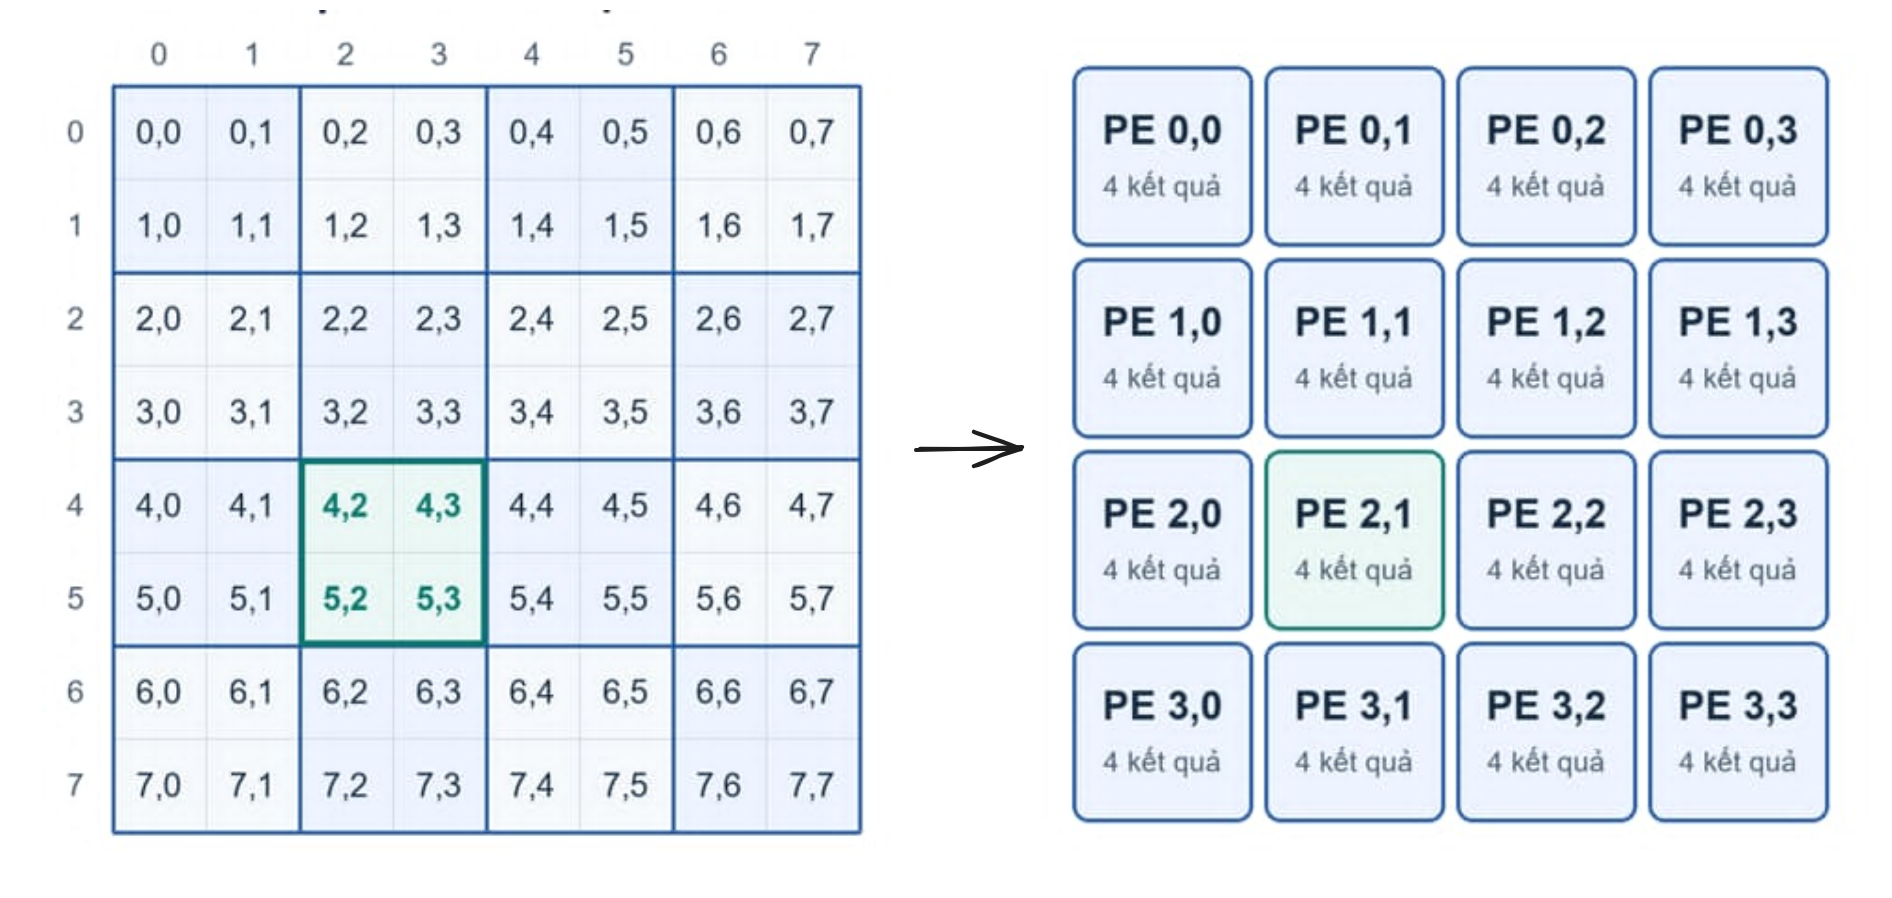
\includegraphics[width=1.0\linewidth]{figures/PE_4x4.png}
        \caption{Mảng PE 4x4}
        \label{fig:placeholder}
    \end{figure}
        
\end{enumerate}

\subsubsection{Phiên bản 1 - Systolic}

Phiên bản Systolic có 16 PE chia thành mảng ($4\times4$). Mỗi PE phụ trách 1 tile kết quả ($2\times2$). Để tái sử dụng các toán hạng, các tile của \textit{A} được truyền giữa các PE trên cùng hàng, còn các tile của \textit{B} được truyền giữa các PE trên cùng cột. Bộ điều khiển phát tile theo lịch lệch nhịp để hai toán hạng tương ứng đến đúng PE trong cùng 1 chu kỳ.

\begin{enumerate}[label=\alph*.]
    \item \textbf{Sơ đồ khối tổng thể}

    Hai ma trận đầu vào được lưu trong 2 bank BRAM đọc đồng bộ. Mỗi bank gồm 16 phần tử, mỗi phần tử chứa 1 tile ($2\times2$) độ rộng 64 bit. Cổng nạp chọn BRAM đích và địa chỉ tile. Khi cả 2 ma trận được nạp đủ, hệ thống có thể nhận lệnh \textit{start}.

    Trong mỗi lượt \textit{K}, bộ điều khiển đọc bốn tile \textit{A} và bốn tile \textit{B} vào các bộ đệm ở biên mảng. Mảng PE nhận các tile từ bộ đệm, thực hiện phép nhân tích lũy và giữ tổng riêng trong RAM cục bộ, Sau lượt cuối, bộ điều khiển chọn PE và vị trí tương ứng để lưu từng phần tử \textit{C}.
    
\begin{figure}[H]
    \centering
    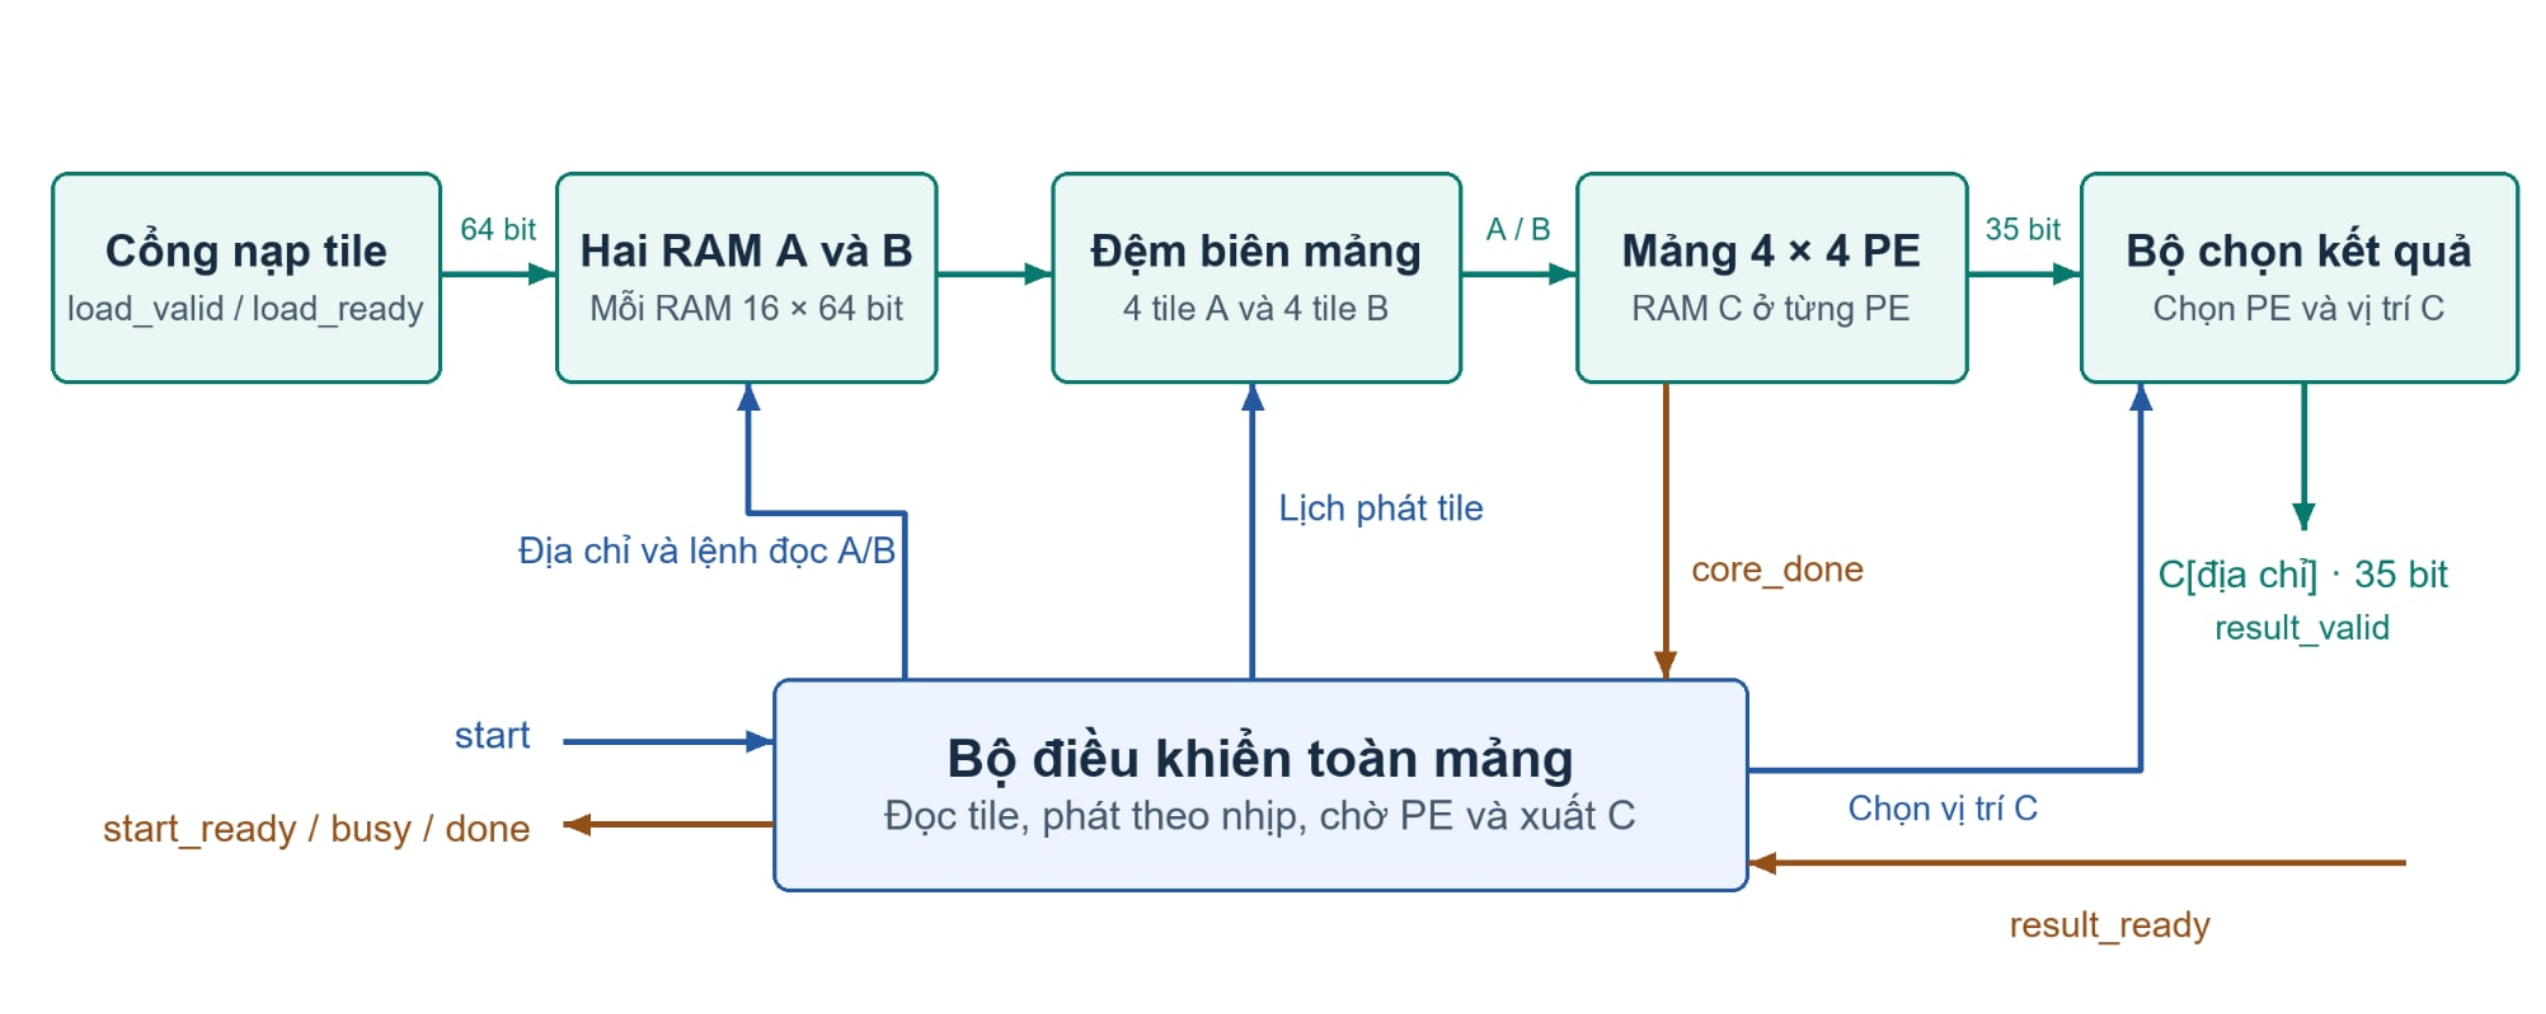
\includegraphics[width=1.0\linewidth]{figures/Systolic_block_diagram.png}
    \caption{Sơ đồ khối bộ nhân ma trận Systolic}
    \label{fig:placeholder}
\end{figure}

    \item \textbf{Kiến trúc phần cứng}

    Với cách đánh số tile theo hàng, tile tại vị trí (r,c) có địa chỉ (4r+c). Ở lượt \textit{K}, bộ điều khiển lần lượt đọc các cặp $A_{s,K}$, $B_{K,s}$. với ($s=0,1,2,3$). Hai bank BRAM được đọc đồng thời cho từng cặp. Địa chỉ đọc RAM \textit{A} là ($4s+K$), còn địa chỉ đọc RAM \textit{B} là ($4K+s$).

    Các tile \textit{A} đi vào từ mép trái và được chuyển sang PE bên phải. Các tile \textit{B} đi vào từ mép trên và được chuyển xuống PE bên dưới. Khi nhận đủ hai tile, mỗi PE chốt dữ liệu để tính toán và chuyển tiếp tile cho PE lân cận ở chu kỳ sau. Quá trình chuyển tiếp diễn ra trong khi PE đang tính. Tổng riêng của tile \textit{C} được giữ tại PE phụ trách qua bốn lượt \textit{K}.
    
\begin{figure}[H]
    \centering
    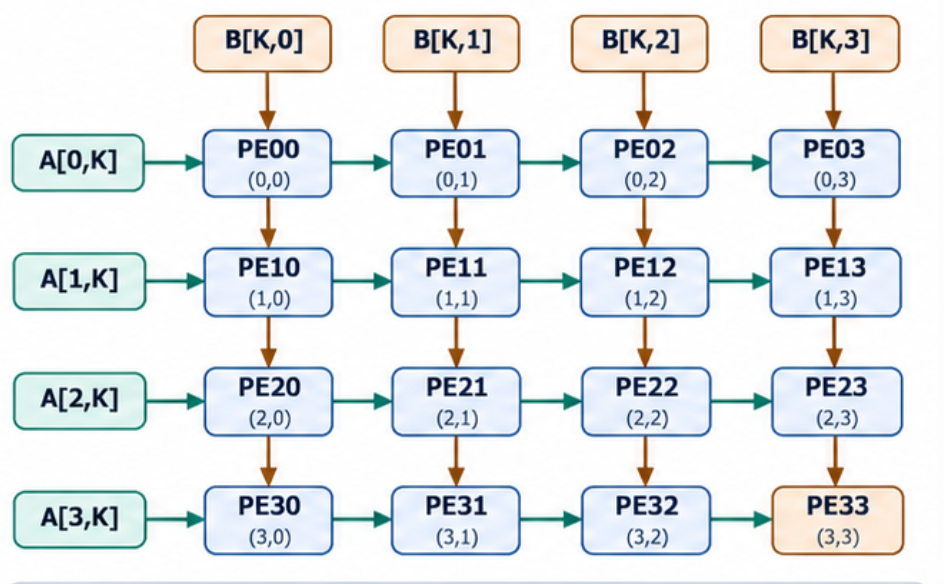
\includegraphics[width=0.8\linewidth]{figures/Systolic_flow.png}
    \caption{Luồn nhận tile của PE của Systolic array}
    \label{fig:placeholder}
\end{figure}

    Mỗi tile đã đọc từ BRAM được sử dụng tại bốn PE. Sau bốn lượt \textit{K}, hệ thống đã đọc 16 tile \textit{A} và 16 tile \textit{B}, tương ứng 128 phần tử đầu vào. Đây là lượng dữ liệu đọc từ hai BRAM đầu vào. Việc chuyển tiếp giữa các PE và truy cập RAM tổng riêng \textit{C} diễn ra bên trong mảng.

    \item \textbf{Lưu đồ thuật toán và FSM}

    Thuật toán bắt đầu tại ($K=0$). Trong mỗi lượt, hệ thống chuẩn bị bốn cặp tile, phát dữ liệu theo lịch và cập nhật tổng riêng tại từng PE. Ở lượt đầu, mỗi PE dùng tích đầu tiên của từng vị trí để khởi tạo tổng. Ở các lượt sau, PE tiếp tục cộng vào giá trị đã lưu. Bộ điều khiển chỉ tăng \textit{K} sau khi nhận đủ tín hiệu hoàn thành từ 16 PE. Sau lượt ($K=3$), hệ thống lần lượt xuất 64 phần tử kết quả theo thứ tự hàng.
    
\begin{figure}[H]
        \centering
        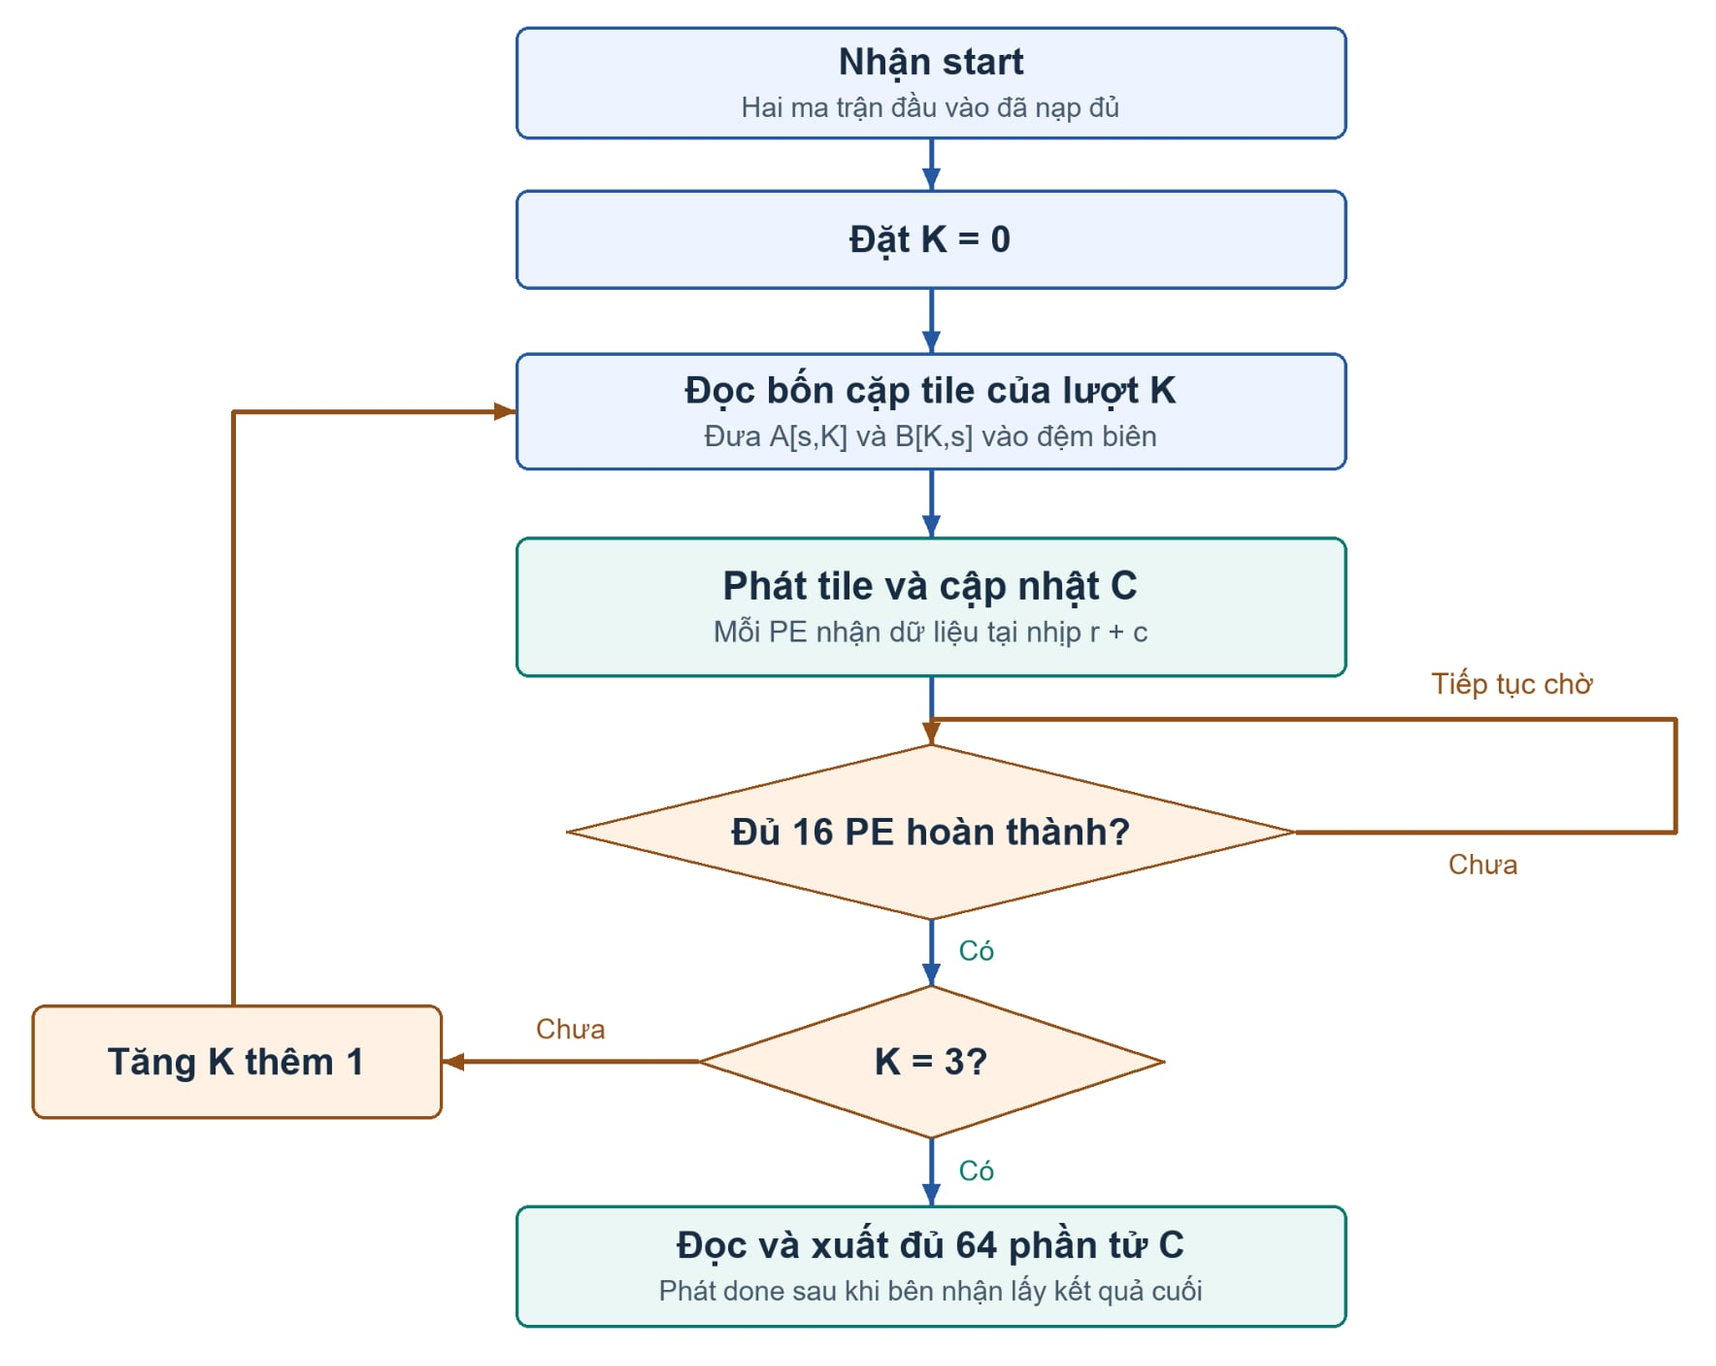
\includegraphics[width=0.8\linewidth]{figures/Systolic_flowchart.png}
        \caption{Lưu đồ thuật toán nhận ma trận theo luồng Systolic}
        \label{fig:placeholder}
\end{figure}

\begin{figure}[H]
    \centering
    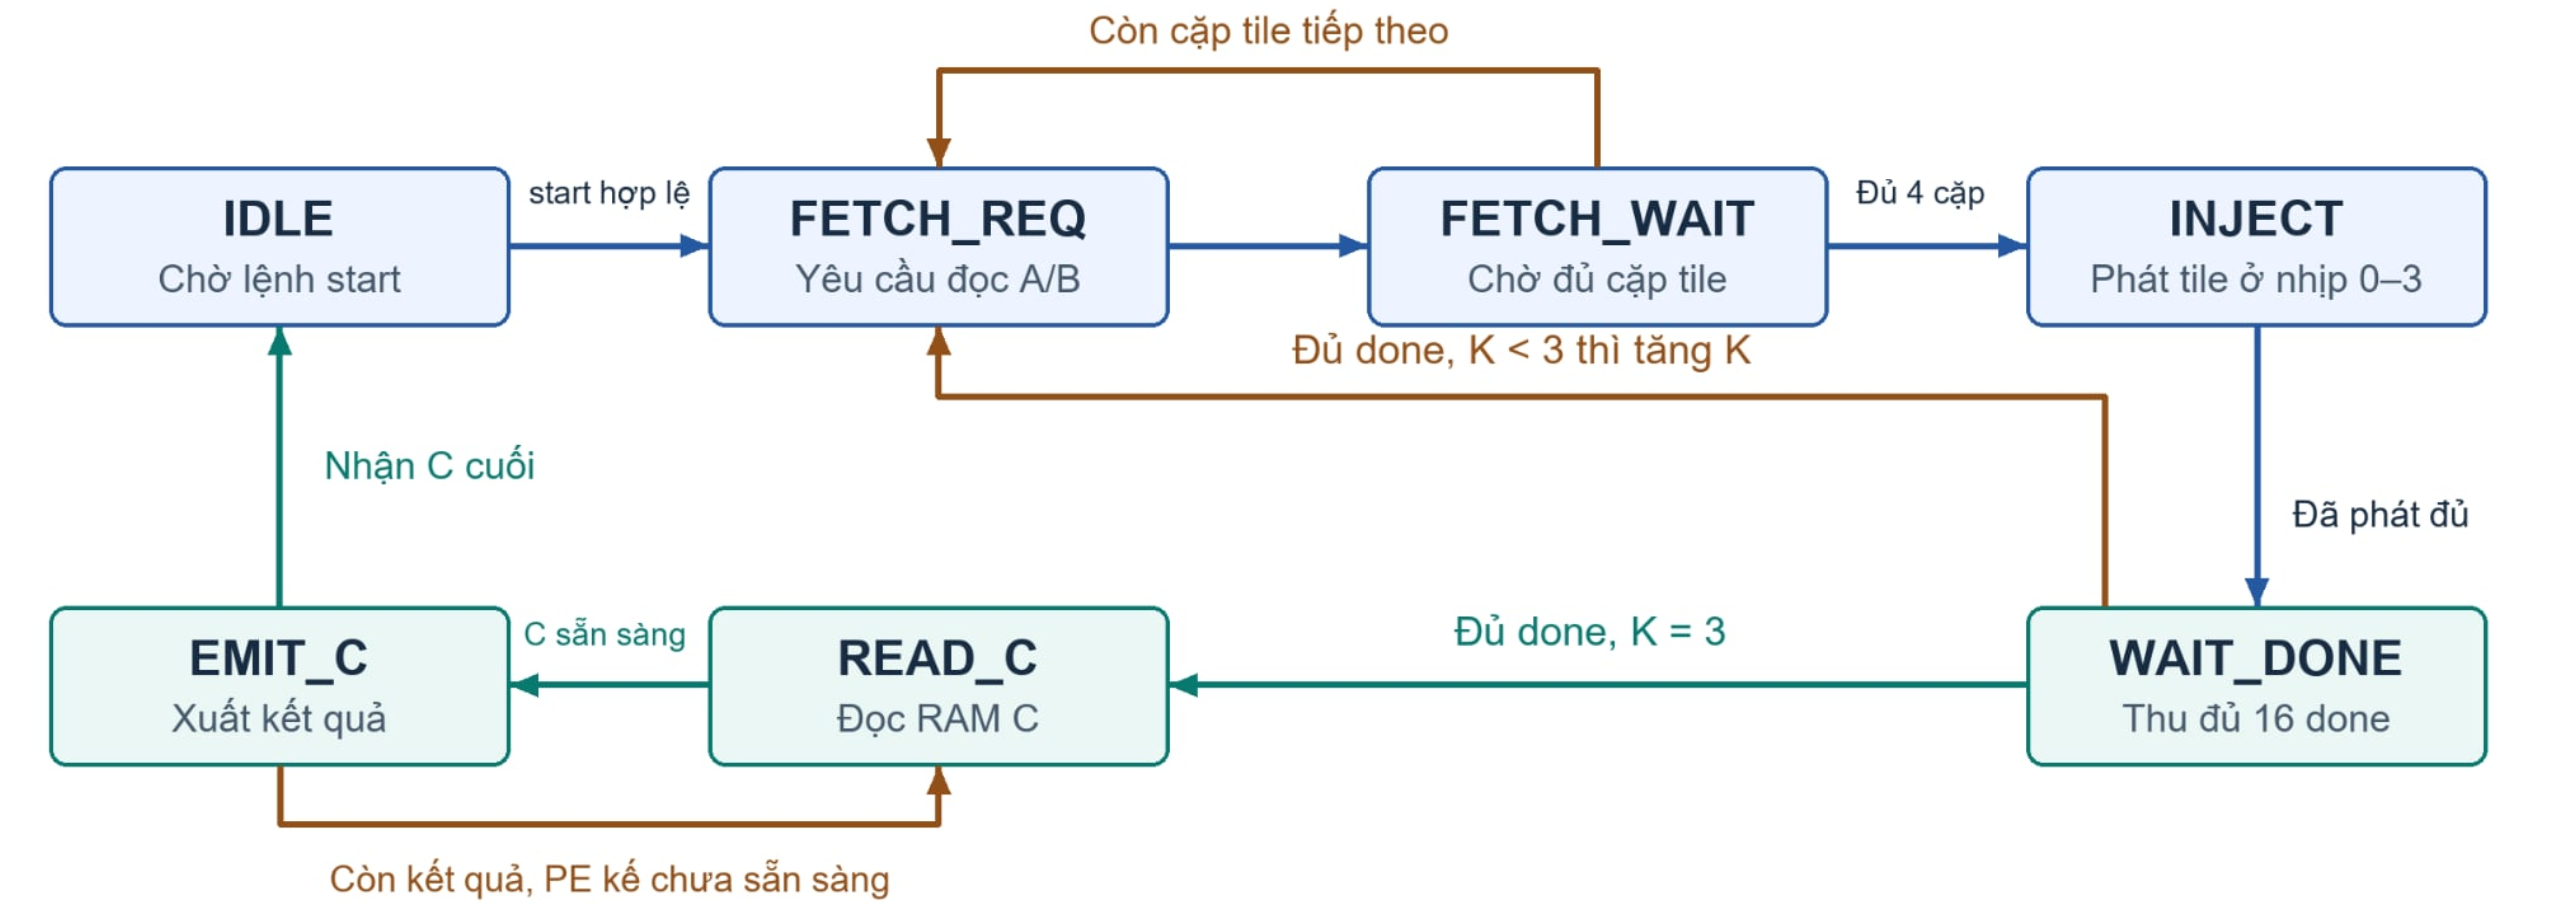
\includegraphics[width=1.0\linewidth]{figures/Systolic_FSM.png}
    \caption{FSM bộ nhân ma trận Systolic}
    \label{fig:placeholder}
\end{figure}
        
\end{enumerate}

\subsubsection{Phiên bản 2 - Multicast}

\section{Thiết kế bộ kiểm thử bằng UART}
\label{sec:kiem_thu_uart}
Để có thể nhập và kiểm thử được phép nhân 2 ma trận hoàn toàn chính xác. Hệ thống này sẽ xây dựng 1 bộ UART cho phép người dùng nhập hai ma trận từ terminal UART của máy tính thông qua một giao diện.
\subsection{Sơ đồ kết nối FPGA với máy tính}

Đầu tiên, thiết lập máy tính kết nối với bộ chuyển đổi CP210x
qua cổng USB. Phía UART của CP210x sử dụng ba dây: TXD, RXD và GND.
Hình~\ref{fig:uart_wiring} trình bày cách đấu dây theo số chân đã
khai báo trong tệp ràng buộc Quartus của thiết kế.

Tuy nhiên DIP SWITCH của board đã được hàn sẵn nên để kiếm chứng được DIP SWITCH nhận đúng tín hiệu đầu vào, chúng ta sẽ sử dụng LED built-in sẵn trên board là LED 01 - LED 04 để chứng minh board và mode chạy đúng.

\begin{figure}[htbp]
    \centering
    \begin{minipage}[b]{0.47\linewidth}
        \centering
        \IfFileExists{figures/dip_switch_board.png}{
            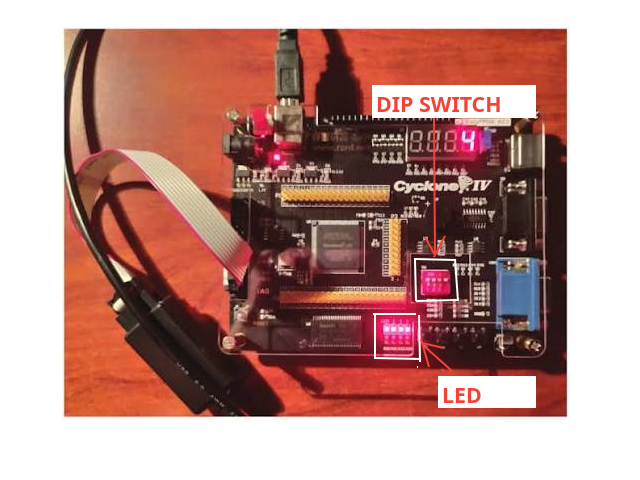
\includegraphics[width=\linewidth,height=4cm,keepaspectratio]
                {figures/dip_switch_board.png}
        }{
            \fbox{\parbox[c][4cm][c]{0.9\linewidth}{
                \centering Ảnh DIP switch trên board
            }}
        }
        \par\smallskip
        \textbf{(a)} DIP switch trên board FPGA
    \end{minipage}
    \hfill
    \begin{minipage}[b]{0.47\linewidth}
        \centering
        \IfFileExists{figures/cp2102_uart.jpg}{
            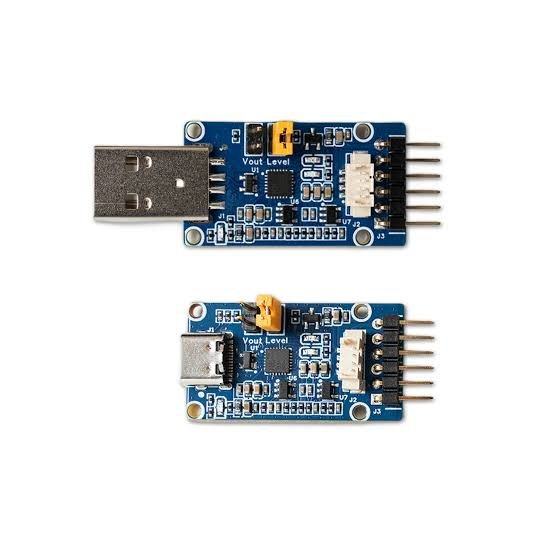
\includegraphics[width=\linewidth,height=4cm,keepaspectratio]
                {figures/cp2102_uart.jpg}
        }{
            \fbox{\parbox[c][4cm][c]{0.9\linewidth}{
                \centering Ảnh module CP2102
            }}
        }
        \par\smallskip
        \textbf{(b)} Bộ chuyển đổi USB--UART CP2102
    \end{minipage}
    \caption{Phần cứng dùng để chọn chế độ và kiểm thử giao tiếp UART.}
    \label{fig:uart_test_hardware}
\end{figure}

\begin{itemize}
    \item \textbf{Cụm công tắc DIP 
    (Hình~\ref{fig:uart_test_hardware}(a)):}
    Được sử dụng để lựa chọn chế độ kiểm tra giao tiếp UART:
    \begin{itemize}
        \item DIP1: Kiểm tra chức năng truyền dữ liệu (TX) của FPGA.
        \item DIP2: Kiểm tra chức năng nhận dữ liệu (RX) của FPGA.
        \item DIP3: Kích hoạt chế độ giao dịch dữ liệu ma trận.
    \end{itemize}

    \item \textbf{Module CP2102 
    (Hình~\ref{fig:uart_test_hardware}(b)):}
    Đóng vai trò chuyển đổi giao tiếp USB--UART giữa máy tính 
    và FPGA. Các kết nối phần cứng được thực hiện như sau:
    \begin{itemize}
        \item TXD $\rightarrow$ \texttt{uart\_rx} 
        của FPGA (\texttt{PIN\_24}).
        \item RXD $\rightarrow$ \texttt{uart\_tx} 
        của FPGA (\texttt{PIN\_114}).
        \item GND: Nối chung mass giữa module CP2102 và FPGA.
    \end{itemize}
\end{itemize}

\begin{figure}[htbp]
\centering
\resizebox{0.98\linewidth}{!}{%
\begin{tikzpicture}[
    x=1mm, y=1mm, >=stealth,
    font=\normalfont\small,
    thietbi/.style={
        draw=black!70, thick, rounded corners=1.5mm
    },
    duonggui/.style={->, thick, draw=blue!65!black},
    duongtra/.style={->, thick, draw=teal!70!black},
    dieukhien/.style={->, thick, draw=orange!55!black},
    chan/.style={font=\normalfont\ttfamily\small},
    nhan/.style={font=\normalfont\footnotesize}
]

    % Bộ chuyển đổi USB--TTL
    \path[thietbi, fill=gray!6] (19,0) rectangle (60,43);
    \node[font=\bfseries] at (39.5,37) {CP210x};
    \node at (39.5,31.5) {Bộ chuyển USB--TTL};

    % FPGA
    \path[thietbi, fill=blue!4] (110,0) rectangle (176,43);
    \node[font=\bfseries] at (143,37) {FPGA Cyclone IV E};
    \node at (143,31.5) {EP4CE6E22C8};

    % Kết nối USB với máy tính
    \node[align=center] at (6,29) {Cổng USB\\máy tính};
    \draw[<->, thick] (1,20) -- (19,20);

    % Cổng UART của CP210x
    \node[chan, anchor=east] at (59,23) {TXD};
    \node[chan, anchor=east] at (59,14) {RXD};
    \node[chan, anchor=east] at (59,5)  {GND};

    % Tên tín hiệu và số chân tương ứng trên FPGA
    \node[chan, anchor=west] at (111,23) {uart\_rx};
    \node[chan, anchor=west] at (111,14) {uart\_tx};
    \node[chan, anchor=west] at (111,5)  {GND};

    \node[chan, anchor=east] at (175,23) {PIN\_24};
    \node[chan, anchor=east] at (175,14) {PIN\_114};

    % Ba dây giữa CP210x và FPGA
    \draw[duonggui] (60,23) -- (110,23);
    \node[nhan, above] at (85,23) {Lệnh và ma trận $A$, $B$};

    \draw[duongtra] (110,14) -- (60,14);
    \node[nhan, above] at (85,14) {Phản hồi và kết quả $C$};

    \draw[thick] (60,5) -- (110,5);
    \node[nhan, above] at (85,5) {GND chung};

    % Cụm DIP trên board: mỗi cột là một công tắc
    \path[thietbi, fill=orange!8] (106,60) rectangle (180,83);
    \node[font=\bfseries] at (143,78.5) {DIP switch trên board};

    \draw[black!35] (106,74) -- (180,74);
    \draw[black!35] (131,60) -- (131,74);
    \draw[black!35] (155,60) -- (155,74);

    \node[chan] at (118.5,70) {DIP1};
    \node[nhan] at (118.5,64.5) {Thử phát TX};

    \node[chan] at (143,70) {DIP2};
    \node[nhan] at (143,64.5) {Thử nhận RX};

    \node[chan] at (167.5,70) {DIP3};
    \node[nhan] at (167.5,64.5) {Nhân ma trận};

    % Các đường chọn chế độ đi vào cạnh trên của FPGA
    \draw[dieukhien] (118.5,60) -- (118.5,43);
    \draw[dieukhien] (143,60)   -- (143,43);
    \draw[dieukhien] (167.5,60) -- (167.5,43);

    \node[fill=white, inner sep=1.5pt, font=\ttfamily\scriptsize]
        at (118.5,51.5) {PIN\_88};
    \node[fill=white, inner sep=1.5pt, font=\ttfamily\scriptsize]
        at (143,51.5) {PIN\_89};
    \node[fill=white, inner sep=1.5pt, font=\ttfamily\scriptsize]
        at (167.5,51.5) {PIN\_90};

\end{tikzpicture}%
}
\caption{Sơ đồ đấu dây UART và các công tắc chọn chế độ kiểm thử.
DIP1 kiểm tra chiều FPGA phát, DIP2 kiểm tra chiều FPGA nhận và
DIP3 kích hoạt chế độ nhân ma trận. Các công tắc tác động ở mức thấp.}
\label{fig:uart_wiring}
\end{figure}

\paragraph*{Đặc tả cơ chế hoạt động trong mỗi mode khi gạt DIP switch}

Ba công tắc DIP trên board cho phép kiểm tra lần lượt đường phát,
đường nhận và giao dịch ma trận qua UART. Khi gạt công tắc sang
vị trí ON, chân đầu vào tương ứng của FPGA ở mức logic 0.
Module \texttt{matmul.sv} đồng bộ tín hiệu theo clock 50~MHz
và lọc dội khoảng 20~ms. Nếu bộ phát đang truyền một ký tự,
hệ thống chờ đến hết stop bit trước khi đổi chế độ.

Khi nhiều công tắc cùng bật, thứ tự ưu tiên là DIP3, DIP2 rồi
DIP1. Trong quy trình kiểm thử dưới đây, mỗi lần chỉ bật một
công tắc để xác định rõ chức năng đang được kiểm tra.

\medskip
\noindent\textbf{Tất cả DIP ở OFF -- \texttt{MODE\_IDLE}.}
Đưa cả ba công tắc về OFF để kiểm tra trạng thái chờ. Các LED
báo chế độ và LED 7 đoạn đều tắt. Đường \texttt{uart\_tx} giữ
mức nghỉ logic 1. Đây cũng là chế độ ban đầu sau reset.

\begin{figure}[H]
    \centering
    \begin{subfigure}[b]{0.47\linewidth}
        \centering
        \dipimage{images/mode_idle_fsm.png}
        \caption{Điều kiện vào và ra khỏi trạng thái chờ.}
        \label{fig:mode_idle_fsm}
    \end{subfigure}
    \hfill
    \begin{subfigure}[b]{0.47\linewidth}
        \centering
        \dipimage{images/mode_idle_evidence.png}
        \caption{Trạng thái DIP và LED trên board.}
        \label{fig:mode_idle_evidence}
    \end{subfigure}
    \caption{Kiểm tra trạng thái chờ khi cả ba DIP ở OFF.}
    \label{fig:mode_idle}
\end{figure}

\noindent\textbf{Bật riêng DIP1 -- \texttt{MODE\_TX}.}
Mở terminal trên máy tính, chọn cổng của CP2102 và cấu hình
9600 baud, 8N1. Khi bật DIP1, LED1 sáng và FPGA liên tục phát
ký tự \texttt{A} (ASCII \texttt{0x41}). Sau khi hoàn tất một
khung UART, bộ phát nạp lại cùng ký tự nếu DIP1 vẫn được chọn.
Kết quả mong đợi là chuỗi \texttt{AAAA...} xuất hiện liên tục
trên cùng một dòng của terminal. Phép thử này kiểm tra chiều
từ TX của FPGA (\texttt{PIN\_114}) đến RXD của CP2102.

\begin{figure}[H]
    \centering
    \begin{subfigure}[b]{0.47\linewidth}
        \centering
        \dipimage{images/mode_tx_fsm.png}
        \caption{Trình tự nạp và phát lặp ký tự \texttt{A}.}
        \label{fig:mode_tx_fsm}
    \end{subfigure}
    \hfill
    \begin{subfigure}[b]{0.47\linewidth}
        \centering
        \dipimage{images/mode_tx_evidence.png}
        \caption{Chuỗi ký tự nhận được trên terminal.}
        \label{fig:mode_tx_evidence}
    \end{subfigure}
    \caption{Kiểm tra chiều truyền từ FPGA đến máy tính bằng DIP1.}
    \label{fig:mode_tx}
\end{figure}

\noindent\textbf{Bật riêng DIP2 -- \texttt{MODE\_RX}.}
Tắt DIP1, bật DIP2 và giữ nguyên cấu hình terminal. Trong chế độ
này, LED2 sáng. Gửi ký tự \texttt{7} từ máy tính và quan sát LED
7 đoạn trên board. Khi bộ thu nhận đủ một khung hợp lệ, tín hiệu
\texttt{rx\_valid} được kích hoạt và LED 7 đoạn hiển thị số 7.
Gửi tiếp ký tự Backspace (\texttt{0x08}) hoặc Delete
(\texttt{0x7F}) để đưa giá trị hiển thị về 0. Phép thử này kiểm
tra chiều từ TXD của CP2102 đến RX của FPGA (\texttt{PIN\_24}).

\begin{figure}[H]
    \centering
    \begin{subfigure}[b]{0.47\linewidth}
        \centering
        \dipimage{images/mode_rx_fsm.png}
        \caption{Trình tự nhận byte và cập nhật chữ số.}
        \label{fig:mode_rx_fsm}
    \end{subfigure}
    \hfill
    \begin{subfigure}[b]{0.47\linewidth}
        \centering
        \dipimage{images/mode_rx_evidence.png}
        \caption{LED 7 đoạn sau khi gửi ký tự \texttt{7}.}
        \label{fig:mode_rx_evidence}
    \end{subfigure}
    \caption{Kiểm tra chiều truyền từ máy tính đến FPGA bằng DIP2.}
    \label{fig:mode_rx}
\end{figure}

\noindent\textbf{Bật riêng DIP3 -- \texttt{MODE\_MATRIX}.}
Sau khi kiểm tra hai chiều UART bằng DIP1 và DIP2, tắt DIP2,
bật DIP3 và đóng terminal để nhường cổng nối tiếp cho GUI.
LED3 sáng, LED 7 đoạn tắt và FPGA kích hoạt bộ điều khiển
\texttt{matrix\_uart}.

Trên GUI, chọn cổng của CP2102 và nhấn \textit{Kết nối}.
Ứng dụng gửi \verb|M 0\n| để đồng bộ. Do kích thước 0 không
hợp lệ, FPGA trả \texttt{ERR} rồi \texttt{READY}; đây là phản hồi
mong đợi ở bước đồng bộ. Tiếp theo, chọn \textit{Mẫu $2\times2$}
và nhấn \textit{Gửi FPGA và đối chiếu}. Với bộ mẫu có sẵn,
giao dịch đạt khi GUI nhận đủ bốn phần tử của
\[
    C =
    \begin{bmatrix}
        19 & 22\\
        43 & 50
    \end{bmatrix},
\]
nhận dòng \texttt{READY} cuối và xác nhận kết quả FPGA khớp
với kết quả Python.

\begin{figure}[H]
    \centering
    \begin{subfigure}[b]{0.47\linewidth}
        \centering
        \dipimage{images/mode_matrix_fsm.png}
        \caption{Trình tự nhận ma trận, tính và trả kết quả.}
        \label{fig:mode_matrix_fsm}
    \end{subfigure}
    \hfill
    \begin{subfigure}[b]{0.47\linewidth}
        \centering
        \dipimage{images/mode_matrix_evidence.png}
        \caption{Kết quả FPGA và Python trên GUI.}
        \label{fig:mode_matrix_evidence}
    \end{subfigure}
    \caption{Kiểm thử giao dịch nhân ma trận bằng DIP3.}
    \label{fig:mode_matrix}
\end{figure}

Hình~\ref{fig:uart_mode_fsm} mô tả cách cập nhật thanh ghi
\texttt{mode}. Sau khi DIP ổn định, nếu bộ phát đang bận
(\texttt{tx\_busy}=1), FPGA giữ chế độ hiện tại đến hết stop bit.
Khi bộ phát rảnh, FPGA chọn chế độ theo thứ tự ưu tiên
\textbf{DIP3, DIP2, DIP1}. Vì vậy, nếu DIP1 và DIP2 cùng bật
thì FPGA chọn \texttt{MODE\_RX}; nếu DIP3 cũng bật thì FPGA chọn
\texttt{MODE\_MATRIX}.

\begin{figure}[htbp]
\centering
\resizebox{0.96\linewidth}{!}{%
\begin{tikzpicture}[
    x=1mm, y=1mm, >=stealth,
    font=\normalfont\small,
    trangthai/.style={
        draw=black!70, thick, rounded corners=2pt,
        minimum width=30mm, minimum height=11mm, align=center
    },
    mui/.style={->, thick},
    day/.style={thick},
    nhan/.style={font=\normalfont\footnotesize, align=center}
]

    % Quy tắc này áp dụng từ bất kỳ giá trị hiện tại nào của mode.
    \node[trangthai, fill=gray!8, minimum width=65mm]
        (current) at (60,40)
        {Chế độ hiện tại\\thanh ghi \texttt{mode}};

    % Nếu UART TX đang phát, giữ nguyên mode.
    \draw[mui] (current.east) -- ++(12,0)
        -- ++(0,12) -| (current.north);
    \node[nhan, above] at (83,52)
        {\texttt{tx\_busy = 1}: giữ nguyên};

    % Nếu TX rảnh, cập nhật mode theo giá trị DIP đã lọc dội.
    \draw[day] (current.south) -- (60,21);
    \node[nhan, anchor=west] at (62,28)
        {\texttt{tx\_busy = 0}};
    \draw[day] (0,21) -- (120,21);

    % Bốn trạng thái được mã hóa trong RTL.
    \node[trangthai, fill=gray!6] (idle) at (0,0)
        {\texttt{MODE\_IDLE}\\Chờ};
    \node[trangthai, fill=blue!6] (tx) at (40,0)
        {\texttt{MODE\_TX}\\Thử phát};
    \node[trangthai, fill=green!7] (rx) at (80,0)
        {\texttt{MODE\_RX}\\Thử nhận};
    \node[trangthai, fill=orange!9] (matrix) at (120,0)
        {\texttt{MODE\_MATRIX}\\Nhân ma trận};

    \draw[mui] (0,21)   -- (idle.north);
    \draw[mui] (40,21)  -- (tx.north);
    \draw[mui] (80,21)  -- (rx.north);
    \draw[mui] (120,21) -- (matrix.north);

    % Điều kiện là vị trí vật lý ON/OFF của công tắc.
    \node[nhan, fill=white] at (0,13)   {Tất cả OFF};
    \node[nhan, fill=white] at (40,13)  {Chỉ DIP1 ON};
    \node[nhan, fill=white] at (80,13)  {DIP2 ON\\DIP3 OFF};
    \node[nhan, fill=white] at (120,13) {DIP3 ON};

    % Reset đưa thanh ghi mode về IDLE.
    \draw[mui] (-24,0) -- (idle.west);
    \node[nhan, above] at (-21,0) {Reset};

\end{tikzpicture}%
}
\caption{Quy tắc chuyển giữa bốn chế độ của FPGA theo DIP switch.
Các điều kiện chuyển áp dụng từ bất kỳ chế độ hiện tại nào.}
\label{fig:uart_mode_fsm}
\end{figure}

Trình tự kiểm thử trên board là bật riêng DIP1 để kiểm tra đường
phát, bật riêng DIP2 để kiểm tra đường nhận, sau đó bật DIP3 để
chạy giao dịch ma trận hai chiều. Cả ba phép thử dùng chung cấu
hình UART được trình bày ở mục tiếp theo.

\subsubsection{Lựa chọn baud rate và cấu hình khung UART}

Trước khi kiểm tra các chế độ DIP, cấu hình cổng nối tiếp trên máy
tính ở 9600 baud, 8 bit dữ liệu, không parity, một stop bit (8N1)
và tắt điều khiển luồng. Giá trị 9600 baud được chọn để khớp với
bộ tạo thời gian bit trong hai module \texttt{uart\_tx} và
\texttt{uart\_rx} của FPGA.

Với clock $f_{\mathrm{clk}}=50$~MHz, số chu kỳ dành cho một bit
được chọn theo baud rate mục tiêu $B$:
\[
    N=\operatorname{round}\!\left(\frac{f_{\mathrm{clk}}}{B}\right),
    \qquad
    B_{\mathrm{thực}}=\frac{f_{\mathrm{clk}}}{N}.
\]
Với $B=9600$, ta có $N=5208$. Trong RTL, bộ đếm chạy từ 0 đến
\texttt{BIT\_LAST = 5207}, tương ứng đúng 5208 chu kỳ cho mỗi bit.
Bộ thu dùng \texttt{HALF\_LAST = 2603} để lấy mẫu gần giữa bit.
Ba thông số thời gian thu được là
\[
    B_{\mathrm{thực}}\approx 9600{,}61~\mathrm{baud},\qquad
    T_{\mathrm{bit}}=104{,}16~\mu\mathrm{s},\qquad
    T_{\mathrm{8N1}}=10T_{\mathrm{bit}}=1{,}0416~\mathrm{ms}.
\]

Khi giữ nguyên clock 50~MHz, tăng $N$ làm mỗi bit kéo dài hơn và
baud rate giảm. Chẳng hạn, để chuyển sang 19200 baud, cần đặt
$N=2604$, đổi \texttt{BIT\_LAST} thành 2603 ở cả bộ phát và bộ thu,
đổi \texttt{HALF\_LAST} thành 1301 ở bộ thu, đồng thời cập nhật
baud rate trên máy tính. Các lựa chọn về parity và stop bit quyết
định số bit trong một khung, do đó ảnh hưởng thời gian truyền một
ký tự. Trong thiết kế 8N1 hiện tại, mỗi ký tự gồm một start bit,
tám bit dữ liệu và một stop bit.

\subsubsection{Kiểm tra đường phát bằng DIP1}

Bật riêng DIP1 và mở terminal nối tiếp ở cấu hình 9600 baud, 8N1.
Ở chế độ này, FPGA liên tục phát ký tự \texttt{A} có mã ASCII
\texttt{0x41}. Khi bộ phát rảnh, \texttt{uart\_tx} nạp ký tự vào
thanh ghi phát. Sau khi phát hết stop bit, bộ phát tiếp tục nạp
ký tự kế tiếp nếu DIP1 vẫn được chọn.

\begin{figure}[htbp]
\centering
\resizebox{0.87\linewidth}{!}{%
\begin{tikzpicture}[
    x=1mm,y=1mm,>=stealth,
    st/.style={draw,rounded corners=2pt,fill=blue!6,
               minimum height=9mm,align=center},
    arr/.style={->,thick}
]
    \node[st] (idle) at (0,0) {Chờ chọn DIP1};
    \node[st] (load) at (48,0) {Nạp \texttt{0x41}};
    \node[st] (send) at (98,0) {Phát khung 8N1};

    \draw[arr] (idle) -- node[above,font=\scriptsize]{DIP1 bật} (load);
    \draw[arr] (load) -- (send);
    \draw[arr] (send.south) -- ++(0,-10)
        -| node[pos=.25,below,font=\scriptsize]
        {Hết stop bit, DIP1 còn bật} (load.south);
    \draw[arr] (send.north) -- ++(0,10)
        -| node[pos=.25,above,font=\scriptsize]
        {Hết khung, tắt DIP1} (idle.north);
\end{tikzpicture}%
}
\caption{Trình tự phát lặp ký tự \texttt{A} khi kiểm tra riêng DIP1.}
\label{fig:uart_dip1_tx}
\end{figure}

Kết quả mong đợi là terminal hiển thị liên tục \texttt{AAAA...}
trên cùng một dòng. Phép thử này kiểm tra đường từ
\texttt{uart\_tx} của FPGA tại \texttt{PIN\_114} đến RXD của CP210x.
Nếu terminal hiển thị ký tự sai, kiểm tra lại baud rate và định dạng
khung trước khi chuyển sang thử chiều nhận.

\subsubsection{Kiểm tra đường nhận bằng DIP2}

Tắt DIP1, bật riêng DIP2 và giữ nguyên cấu hình terminal. Gửi ký tự
\texttt{7} từ máy tính. Dữ liệu đi từ TXD của CP210x đến
\texttt{uart\_rx} tại \texttt{PIN\_24}. Khi nhận được một khung hợp
lệ, bộ thu phát xung \texttt{rx\_valid}; mạch hiển thị dùng byte vừa
nhận để cập nhật LED 7 đoạn.

\begin{figure}[htbp]
\centering
\resizebox{0.92\linewidth}{!}{%
\begin{tikzpicture}[
    x=1mm,y=1mm,>=stealth,
    st/.style={draw,rounded corners=2pt,fill=green!7,
               minimum height=9mm,align=center},
    arr/.style={->,thick}
]
    \node[st] (wait) at (0,0) {Chờ byte hợp lệ};
    \node[st] (show) at (71,11) {Hiển thị chữ số};
    \node[st] (clear) at (71,-11) {Đưa hiển thị về 0};

    \draw[arr] (wait.north east) --
        node[above,sloped,font=\scriptsize]
        {ASCII \texttt{0} đến \texttt{9}} (show.west);
    \draw[arr] (wait.south east) --
        node[below,sloped,font=\scriptsize]
        {Backspace hoặc Delete} (clear.west);

    \draw[arr] (show.north) -- ++(0,8) -| (wait.north);
    \draw[arr] (clear.south) -- ++(0,-8) -| (wait.south);
\end{tikzpicture}%
}
\caption{Xử lý byte nhận trong chế độ DIP2. Các ký tự khác giữ
nguyên chữ số đang hiển thị.}
\label{fig:uart_dip2_rx}
\end{figure}

LED 7 đoạn phải hiển thị số 7. Nhấn Enter thì số 7 vẫn giữ nguyên;
gửi Backspace (\texttt{0x08}) hoặc Delete (\texttt{0x7F}) thì
màn hình trở về 0. Việc quan sát trực tiếp trên board xác nhận FPGA
đã nhận đúng byte từ máy tính.

\subsubsection{Kiểm thử phép nhân ma trận bằng DIP3}

Sau khi DIP1 xác nhận chiều FPGA phát và DIP2 xác nhận chiều FPGA
nhận, bật riêng DIP3 để kiểm tra hai chiều trong cùng một giao dịch.
Đóng terminal để giải phóng cổng nối tiếp, sau đó mở GUI và chọn
đúng cổng. Ở chế độ này, LED3 sáng và LED 7 đoạn tắt.

\begin{figure}[htbp]
\centering
\resizebox{0.97\linewidth}{!}{%
\begin{tikzpicture}[
    x=1mm,y=1mm,>=stealth,
    st/.style={draw,rounded corners=2pt,fill=orange!9,
               minimum height=10mm,align=center},
    arr/.style={->,thick}
]
    \node[st] (ready) at (0,0) {Phát \texttt{READY}\\và chờ lệnh};
    \node[st] (recv)  at (42,0) {Nhận kích thước\\và ma trận $A,B$};
    \node[st] (run)   at (85,0) {Nạp bộ nhân\\và tính $C$};
    \node[st] (reply) at (125,0) {Phát ma trận $C$\\qua UART};

    \draw[arr] (ready) -- node[above,font=\scriptsize]{\texttt{M}} (recv);
    \draw[arr] (recv) -- node[above,font=\scriptsize]{Đủ dữ liệu} (run);
    \draw[arr] (run) -- node[above,font=\scriptsize]{Hoàn tất} (reply);
    \draw[arr] (reply.south) -- ++(0,-10)
        -| node[pos=.25,below,font=\scriptsize]
        {Đã gửi hàng cuối} (ready.south);
    \draw[arr] (recv.north) -- ++(0,10)
        -| node[pos=.25,above,font=\scriptsize]
        {Dữ liệu lỗi: phát \texttt{ERR}} (ready.north);
\end{tikzpicture}%
}
\caption{Các giai đoạn của một giao dịch ma trận khi bật DIP3.}
\label{fig:uart_dip3_matrix}
\end{figure}

Khi kết nối, GUI gửi \verb|M 0\n| để đồng bộ. Do kích thước 0
không hợp lệ, FPGA đi theo nhánh lỗi trong
Hình~\ref{fig:uart_dip3_matrix}, phát \texttt{ERR} rồi
\texttt{READY}. Đây là phản hồi mong đợi ở bước đồng bộ.
Tiếp theo, chọn mẫu $2\times2$ và nhấn
\textit{Gửi FPGA và đối chiếu}. Phép thử đạt khi GUI nhận đủ
bốn phần tử của $C$, nhận dòng \texttt{READY} cuối và xác nhận
từng giá trị khớp với kết quả Python.

\subsection{Giao diện nạp ma trận, tính toán và đọc kết quả}

\subsubsection{Giao diện trên máy tính}

Giao diện được viết bằng PyQt5 trong tệp \texttt{matrix\_gui.py}.
Người dùng chọn ba kích thước $M$, $K$, $N$, sau đó nhập ma trận
$A_{M\times K}$ và $B_{K\times N}$. Mỗi hàng được nhập trên một
dòng, các phần tử phân cách bằng khoảng trắng. Mỗi kích thước nhận
giá trị từ 1 đến 8. Đối với bài toán chính của đề tài, chọn
$M=K=N=8$.

\begin{figure}[htbp]
    \centering
    \includegraphics[width=0.94\linewidth]{figures/matrix_gui_2x2.png}
    \caption{Giao diện với bộ mẫu $2\times2$. Hai ô phía trên chứa
    ma trận đầu vào. Ở thời điểm chụp, GUI đã tính kết quả Python
    và đang ở trạng thái chưa kết nối FPGA.}
    \label{fig:uart_matrix_gui}
\end{figure}

\begin{itemize}
    \item \textbf{Kết nối và đồng bộ.}
    Sau khi người dùng chọn cổng và nhấn \textit{Kết nối}, GUI gửi
    \verb|M 0\n|. Kích thước 0 khiến FPGA trả hai dòng \texttt{ERR}
    rồi \texttt{READY}. GUI nhận đúng thứ tự này để xác nhận phiên
    làm việc đã đồng bộ. Thời hạn chờ là 5 giây.

    \item \textbf{Tính kết quả tham chiếu.}
    Nút \textit{Tính Python} kiểm tra số hàng, số cột và miền giá trị
    $[-32768,32767]$ của từng phần tử, sau đó hiển thị
    $C_{\mathrm{ref}}=A\cdot B$. Chức năng này có thể sử dụng trước
    khi kết nối board.

    \item \textbf{Gửi và đối chiếu.}
    Nút \textit{Gửi FPGA và đối chiếu} tính lại $C_{\mathrm{ref}}$
    từ dữ liệu hiện tại rồi gửi yêu cầu qua UART. Khi nhận đủ ma trận
    $C$ và dòng \texttt{READY} cuối, GUI so sánh từng ô. Nếu có sai
    lệch, giao diện hiển thị số ô sai, tọa độ ô sai đầu tiên và hai
    giá trị tương ứng. Thời hạn chờ giao dịch là 15 giây.
\end{itemize}
\subsubsection{Định dạng dữ liệu và ví dụ giao dịch}

Sau khi chuyển sang chế độ DIP3 và đồng bộ với FPGA, GUI gửi yêu cầu
nhân ma trận dưới dạng văn bản ASCII. Dòng đầu bắt đầu bằng ký tự
lệnh \texttt{M} (mã \texttt{0x4D}), theo sau là ba kích thước
$M$, $K$, $N$ của phép nhân $A_{M\times K}B_{K\times N}$.
Tiếp theo, GUI gửi $M K$ phần tử của $A$ rồi đến $K N$ phần tử
của $B$, theo thứ tự từng hàng. Hai số trên cùng một hàng được
phân cách bằng dấu cách và mỗi hàng kết thúc bằng ký tự LF
(\texttt{0x0A}).

FPGA phân biệt dữ liệu của hai ma trận bằng số phần tử đã nhận.
Sau khi ghi đủ $M K$ phần tử vào RAM $A$, bộ điều khiển tự chuyển
sang nhận $B$. Vì vậy, GUI chỉ gửi giá trị các phần tử trong phần
dữ liệu. Ký tự \texttt{A} phát lặp ở chế độ DIP1 chỉ dùng để kiểm
tra đường truyền từ FPGA đến máy tính.

\begin{figure}[htbp]
    \centering
    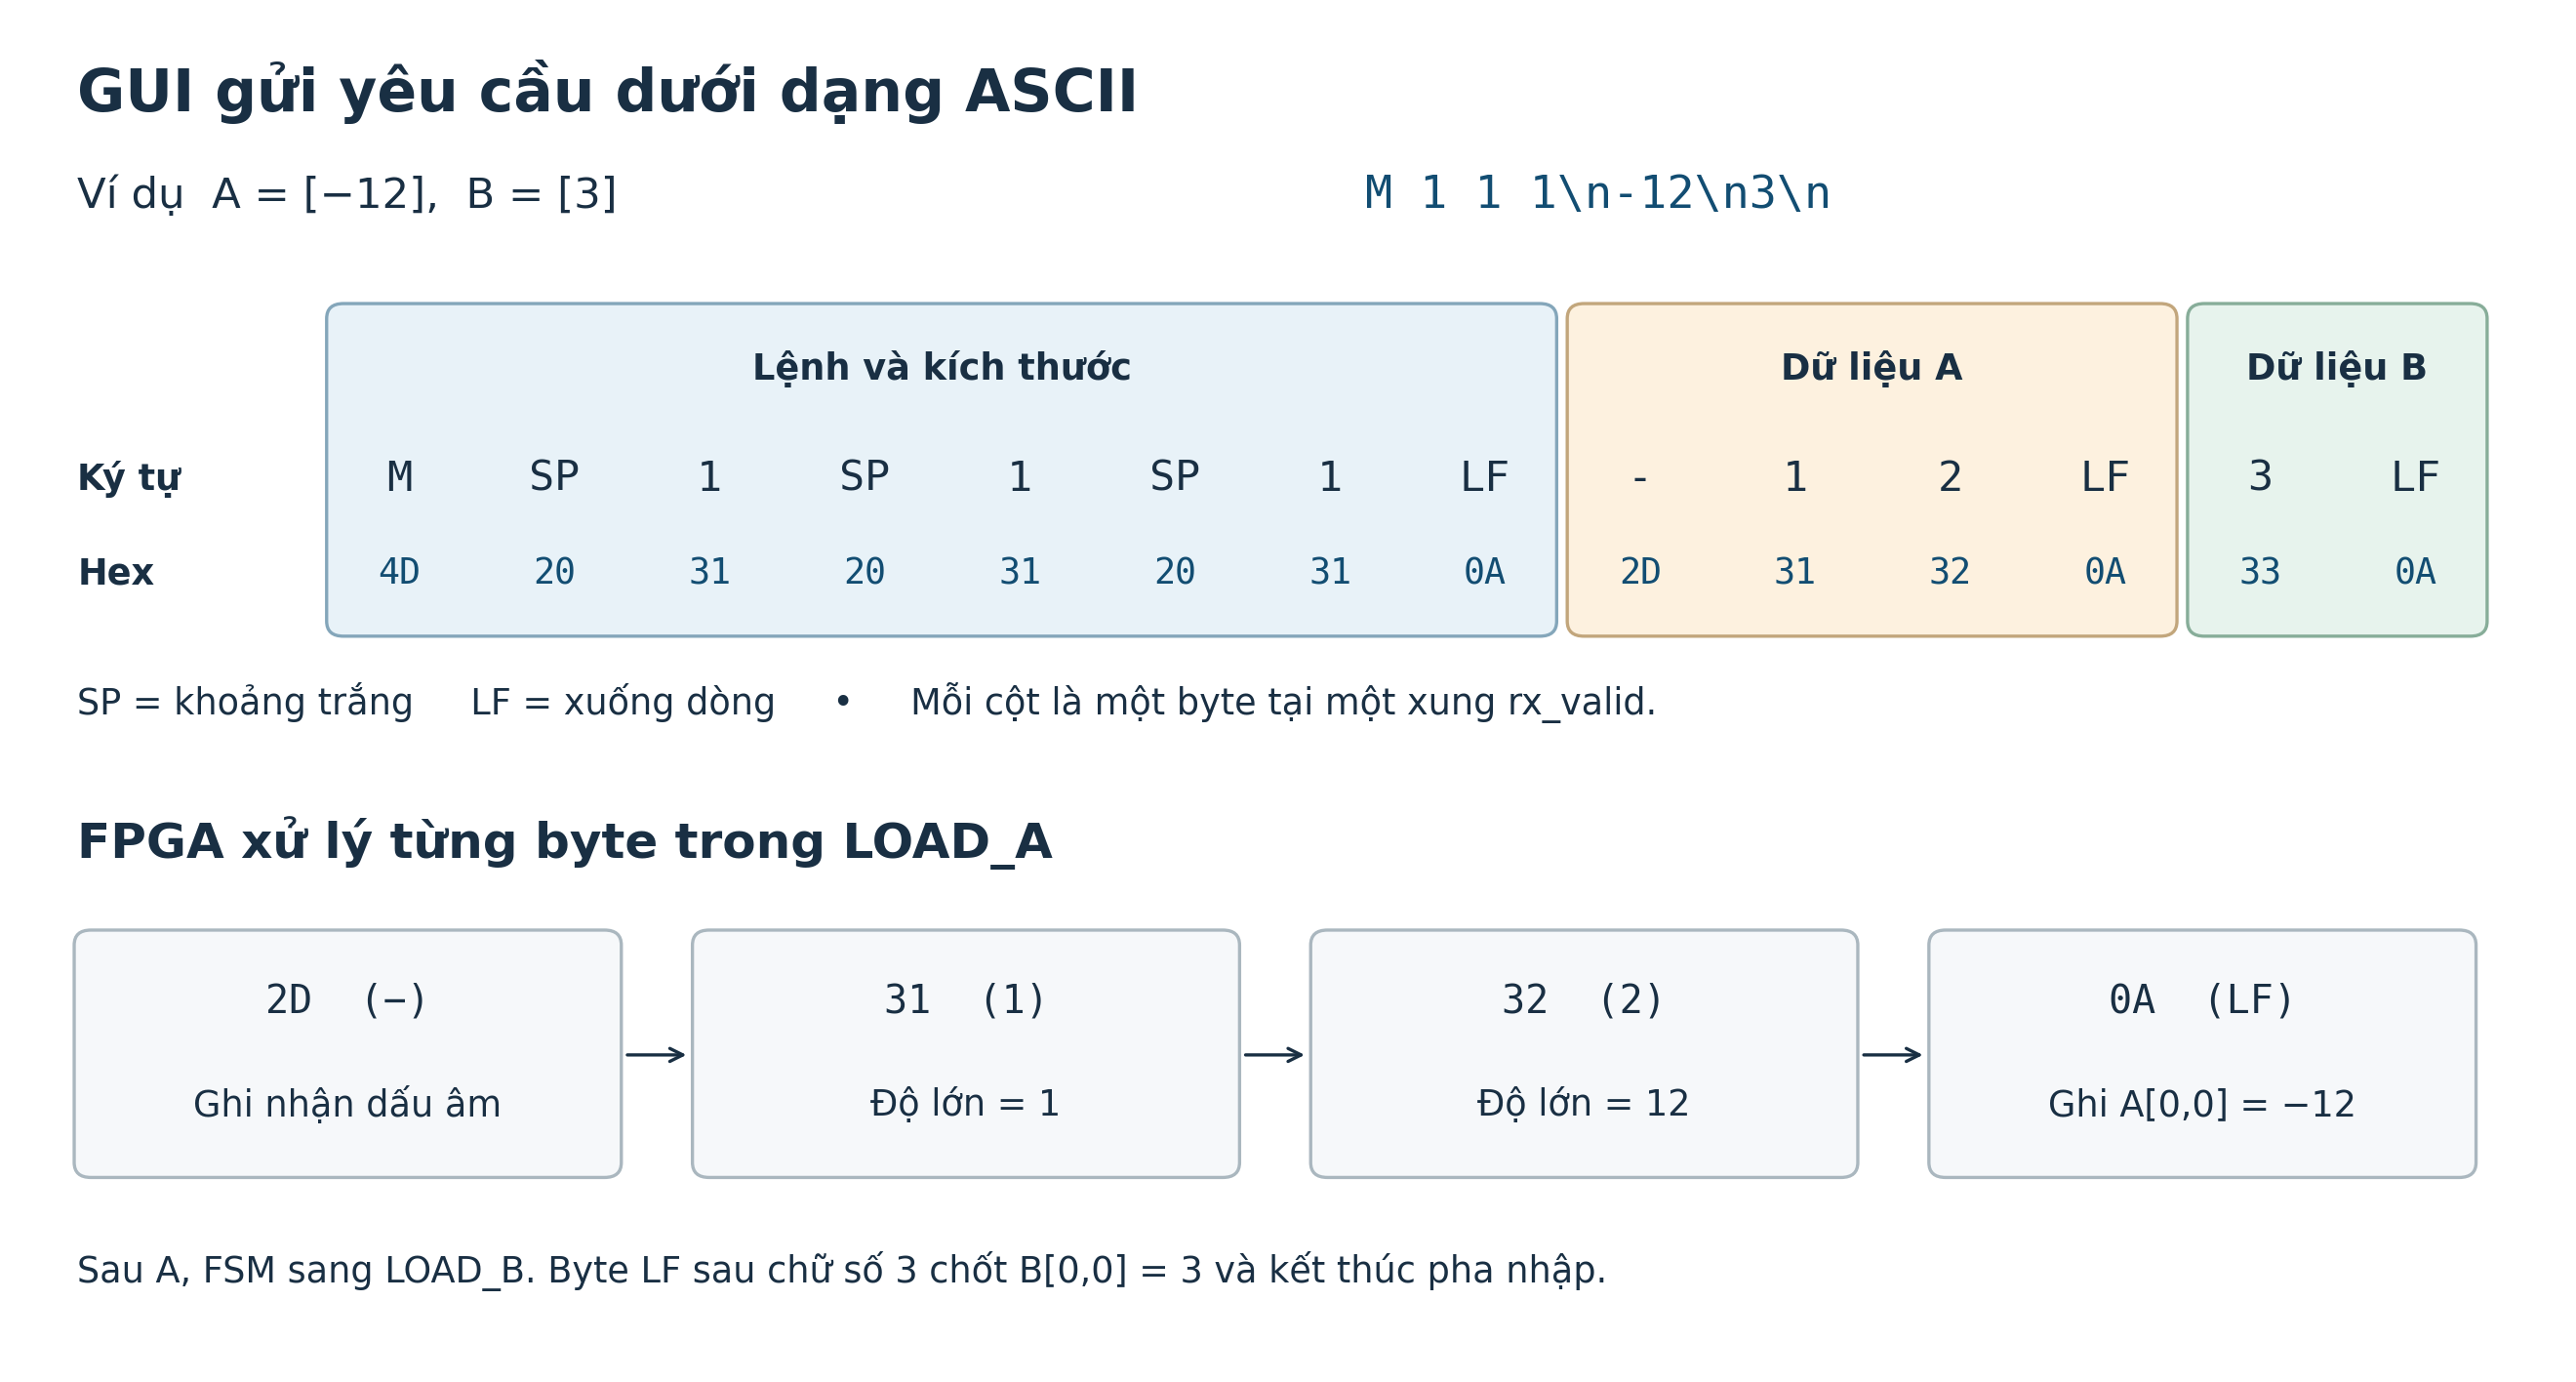
\includegraphics[width=0.98\linewidth]{figures/uart_ascii_parser.png}
    \caption{Giải mã bản tin ASCII cho $A=[-12]$ và $B=[3]$.
    Mỗi cột biểu diễn một byte. SP là dấu cách và LF là ký tự xuống dòng.}
    \label{fig:uart_ascii_parser}
\end{figure}

Trong Hình~\ref{fig:uart_ascii_parser}, GUI gửi chuỗi
\verb|M 1 1 1\n-12\n3\n| gồm 14 byte. Mỗi cụm \verb|\n| trong
cách viết này biểu diễn một byte LF. Riêng phần tử $-12$ cần ba
ký tự ASCII để biểu diễn giá trị và một ký tự LF để chốt số:

\begin{itemize}
    \item \texttt{0x2D} là dấu trừ. Bộ giải mã ghi nhận số đang
    nhập có dấu âm.
    \item \texttt{0x31} và \texttt{0x32} là các chữ số 1 và 2.
    Với mỗi chữ số $d$, bộ giải mã cập nhật độ lớn theo
    $v\leftarrow 10v+d$. Giá trị $v$ lần lượt bằng 1 rồi bằng 12.
    \item \texttt{0x0A} kết thúc số. Bộ điều khiển áp dụng dấu
    và ghi $-12$ vào RAM $A$ dưới dạng số bù hai 16 bit
    (\texttt{0xFFF4}). Hai byte tiếp theo, \texttt{0x33} và
    \texttt{0x0A}, chốt giá trị 3 vào RAM $B$.
\end{itemize}

Bảng~\ref{tab:uart_example} trình bày giao dịch của bộ mẫu
$2\times2$ trên GUI theo thứ tự thời gian.

\begin{table}[htbp]
\centering
\caption{Trình tự trao đổi UART khi nhân hai ma trận $2\times2$}
\label{tab:uart_example}
\small
\begin{tabularx}{\linewidth}{@{}l l X@{}}
\toprule
\textbf{Chiều truyền} & \textbf{Dòng ASCII} & \textbf{Ý nghĩa} \\
\midrule
PC $\to$ FPGA & \texttt{M 2 2 2} & Lệnh nhân với $M=K=N=2$. \\
PC $\to$ FPGA & \texttt{1 2}     & Hàng đầu của $A$. \\
PC $\to$ FPGA & \texttt{3 4}     & Hàng cuối của $A$. \\
PC $\to$ FPGA & \texttt{5 6}     & Hàng đầu của $B$. \\
PC $\to$ FPGA & \texttt{7 8}     & LF sau số 8 chốt phần tử cuối của $B$. \\
\midrule
FPGA $\to$ PC & \texttt{C 2 2}   & Kết quả có hai hàng và hai cột. \\
FPGA $\to$ PC & \texttt{19 22}   & Hàng đầu của $C$. \\
FPGA $\to$ PC & \texttt{43 50}   & Hàng cuối của $C$. \\
FPGA $\to$ PC & \texttt{READY}   & Kết thúc giao dịch, sẵn sàng nhận lệnh mới. \\
\bottomrule
\end{tabularx}
\end{table}

Chẳng hạn, giá trị 19 ở hàng kết quả đầu tiên tương ứng với
$C_{0,0}=1\times5+2\times7$. Mỗi dòng do FPGA phát kết thúc bằng
CR/LF (\texttt{0x0D}, \texttt{0x0A}). GUI kiểm tra kích thước,
nhận đủ hai hàng và chờ dòng \texttt{READY} cuối trước khi đối
chiếu bốn phần tử với kết quả Python.

\subsubsection{Trình tự xử lý trong FPGA}

Module \texttt{uart\_rx} tiếp nhận khung 8N1 và xuất một byte trên
\texttt{rx\_data}. Khi stop bit hợp lệ, tín hiệu \texttt{rx\_valid}
lên mức 1 trong một chu kỳ clock. Bộ điều khiển
\texttt{matrix\_uart} sử dụng xung này để xử lý từng ký tự theo
trạng thái hiện tại của FSM.

\begin{enumerate}
    \item \textbf{Giải mã lệnh và ghi RAM đầu vào.}
    Từ \texttt{WAIT\_M}, ký tự lệnh đưa FSM sang
    \texttt{DIM\_M}, \texttt{DIM\_K} rồi \texttt{DIM\_N} để nhận
    ba kích thước. Trong \texttt{LOAD\_A} và \texttt{LOAD\_B},
    FSM ghép các chữ số như minh họa ở
    Hình~\ref{fig:uart_ascii_parser}. Khi gặp dấu phân cách sau
    một số hợp lệ, FSM ghi phần tử vào địa chỉ $8r+c$, với $r,c$
    là chỉ số hàng và cột tính từ 0. Trên waveform,
    \texttt{rx\_valid} đánh dấu một byte vừa nhận, còn
    \texttt{accept\_token} trong trạng thái nạp đánh dấu thời điểm
    phần tử được ghi vào RAM.

    \item \textbf{Đóng gói dữ liệu và khởi chạy bộ nhân.}
    Sau khi chốt phần tử cuối của $B$, FSM lần lượt thực hiện
    \texttt{TILE\_READ}, \texttt{TILE\_PACK} và \texttt{TILE\_LOAD}.
    Bốn phần tử 16 bit tạo thành một gói 64 bit. Bộ điều khiển nạp
    16 gói cho $A$ rồi 16 gói cho $B$; các ô ngoài kích thước yêu
    cầu được điền 0. Tại \texttt{CORE\_START}, bộ nhân nhận lệnh
    khi \texttt{core\_start\_ready} bằng 1. Cả hai kiến trúc dùng
    cùng giao diện nạp này; bên trong lõi baseline, một MAC vẫn
    xử lý lần lượt từng phần tử.

    \item \textbf{Thu kết quả nhị phân.}
    Trong \texttt{CORE\_WAIT}, mỗi cạnh clock có
    \texttt{core\_result\_valid} bằng 1 tương ứng với một lần ghi
    kết quả 35 bit vào RAM $C$ tại địa chỉ do bộ nhân cung cấp.
    Do lõi xử lý khung $8\times8$, bộ điều khiển thu đủ 64 giá trị,
    kể cả khi GUI yêu cầu phép nhân $2\times2$. Khi nhận
    \texttt{core\_done}, FSM chuyển sang \texttt{HEADER}.

    \item \textbf{Định dạng và phát phản hồi.}
    FSM phát dòng kích thước \texttt{C} kèm $M$, $N$, rồi đọc
    $M\times N$ phần tử cần trả từ RAM $C$. Đối với mỗi phần tử,
    FSM lưu dấu, chuyển trị tuyệt đối sang BCD trong 35 chu kỳ
    và phát từng chữ số ASCII qua \texttt{uart\_tx}. Dấu trừ
    được phát trước chữ số nếu giá trị âm. Sau hàng cuối, FPGA
    gửi dòng \texttt{READY} để kết thúc giao dịch.
\end{enumerate}

\paragraph{Mốc đo khi kiểm thử.}
Trong ca mô phỏng \texttt{FINAL\_1\_UART\_8x8} của kiến trúc
multicast ở 50~MHz, mốc hoàn tất nhập liệu là cạnh clock tại đó
\texttt{accept\_token} chốt phần tử cuối trong \texttt{LOAD\_B}.
Từ mốc này, hệ thống mất 290 chu kỳ để nạp dữ liệu và đưa bộ nhân
đến cạnh nhận \texttt{start}, sau đó mất thêm 121 chu kỳ để nhận đủ
64 kết quả. Như vậy, thời gian từ khi chốt đầu vào đến khi RAM $C$
của \texttt{matrix\_uart} có đủ kết quả là
\[
    (290+121)\times20~\mathrm{ns}
    = 411\times20~\mathrm{ns}
    = 8{,}220~\mu\mathrm{s}.
\]
Riêng khoảng từ \texttt{start} đến lần nhận kết quả thứ 64 là
$2{,}420~\mu\mathrm{s}$. Khi đo toàn bộ giao dịch trên đường UART,
từ start bit đầu của yêu cầu đến hết stop bit của byte LF cuối
trong dòng \texttt{READY}, kết quả là $607{,}214$~ms đối với bộ
dữ liệu này. Thời gian toàn giao dịch phụ thuộc số ký tự ASCII
cần truyền, bao gồm chữ số, dấu âm và ký tự phân cách.
\section{Kiểm chứng và so sánh}

\subsection{Kiểm chứng bằng testbench}

\subsection{So sánh}

\subsubsection{Số chu kỳ xử lý}

\subsubsection{Tài nguyên sử dụng}

\subsubsection{Năng lượng tiêu thụ}
\section{Kết luận và hướng phát triển}

\subsection{Kết quả đạt được}

\subsection{Hướng cải tiến}

% ============================================================
% 13. REFERENCES
% ============================================================

\clearpage
\phantomsection
\addcontentsline{toc}{section}{TÀI LIỆU THAM KHẢO}

\begin{thebibliography}{80}

\bibitem{CVX}
CVX Introduction,
\textit{What is CVX},
\url{http://cvxr.com/cvx/doc/intro.html/},
lần truy cập cuối: 15/04/2017.

\end{thebibliography}

% ============================================================
% END DOCUMENT
% ============================================================

\end{document}
